\documentclass[11pt,a4paper]{article}

\usepackage[utf8]{inputenc}
\usepackage[T1]{fontenc}
\usepackage{amsmath,amssymb,amsthm}
\usepackage{geometry}
\usepackage{hyperref}
\usepackage{enumitem}
\usepackage{booktabs}
\usepackage{graphicx}
\usepackage{mathtools}

\geometry{margin=1in}

\newtheorem{theorem}{Theorem}[section]
\newtheorem{proposition}[theorem]{Proposition}
\newtheorem{lemma}[theorem]{Lemma}
\newtheorem{corollary}[theorem]{Corollary}
\newtheorem{conjecture}[theorem]{Conjecture}
\theoremstyle{definition}
\newtheorem{definition}[theorem]{Definition}
\newtheorem{remark}[theorem]{Remark}

\DeclareMathOperator{\tr}{tr}
\DeclareMathOperator{\diag}{diag}
\DeclareMathOperator{\diam}{diam}
\DeclareMathOperator{\GAP}{GAP}
\DeclareMathOperator{\ReLU}{ReLU}

\title{The Geometric Origin of the Expressivity--Stability Tradeoff\\
in Deep Networks: Non-normal Operator Curvature,\\
Transient Amplification, and Confident Hallucination}

\author{Zeta Hoi-Ho Cheng}

\date{\today \quad (Draft)}

\begin{document}
\maketitle

\begin{abstract}
Why do deep networks hallucinate, and why are some hallucinations
expressed with high confidence? We show that both phenomena have a
\emph{geometric} origin in the non-normality of layer Jacobians.
Every core component of modern Transformers---affine--ReLU layers,
attention operators, and feed-forward blocks---produces Jacobians
whose Hermitian and skew-Hermitian parts fail to commute, generating
nonzero curvature $R(T) = [H,K]$. Drawing on the Petermann excess
noise factor in laser physics and transient growth theory in fluid
mechanics, we prove an \textbf{Expressivity--Stability No-Go Theorem}:
transient amplification (the geometric basis of expressivity) and
excess noise sensitivity (the geometric basis of instability) are
inseparable---both are controlled by operator non-normality.

We introduce \textbf{Projection Residual Connections (PRC)} as a
controllable experimental tool for probing the expressivity--stability
tradeoff. On CIFAR-10, forced normalization causes a 3\% accuracy
drop ($p = 0.006$), confirming that non-normality is necessary for
expressivity. On WikiText-103, forced normalization degrades
perplexity by 19\% ($p = 0.0006$) while simultaneously producing
the \emph{lowest} confidence on errors---exactly as the No-Go
theorem predicts. Destructive PRC ($\beta < 0$) triggers a
\textbf{curvature inflation} effect confirmed across 3~seeds
($p = 0.0012$): the model compensates for suppression by developing
higher non-normality elsewhere, ultimately \emph{increasing}
confidence on errors. This waterbed effect demonstrates that uniform
noise suppression is fundamentally insufficient.

We further test a \textbf{targeted noise discriminator} that learns
to identify amplified noise. Applied post-hoc to frozen weights
(Group~G), the discriminator detects noise (accuracy 68.7\%) but
the gate converges to near-zero---a null result revealing tight
signal--noise entanglement. Applied during training (Group~H),
the discriminator reduces confidence on errors by 20.1\%
($p = 0.0001$) and high-confidence errors by 52.5\%
($p = 0.0010$) with no PPL penalty, achieving lower ConfOnErr
than even the forced-normal model while preserving expressivity.
The gate again decays to zero, but the representations shaped
during co-training persist---the discriminator acts as a transient
training signal rather than an inference-time gate. A controlled noise injection experiment reveals that the
most dangerous noise is not the most non-normal: spectrally
persistent noise without transient amplification doubles
high-confidence errors, while highly non-normal noise with
transient growth reduces them by 86\%---transient amplification
provides an implicit detection signal that aids confidence
recalibration. The geometric perspective reframes hallucination
as having an irreducible, architecture-level component: the
No-Go theorem sets a lower bound, PRC reveals the tradeoff
landscape, the discriminator experiments delineate when targeted
intervention succeeds, and the noise injection experiment
identifies the specific noise geometry that drives confident
hallucination.
\end{abstract}

\tableofcontents

%% ====================================================================
\section{Introduction}
%% ====================================================================

Deep learning architectures rely on residual connections to enable gradient flow
through many layers. The standard residual update
\[
  h_l = h_{l-1} + f_l(h_{l-1})
\]
accumulates all layer outputs with fixed unit weights. While this design enables
training of deep networks, it introduces two interrelated problems:

First, as depth $L$ grows, the accumulated hidden state magnitude grows without bound
under PreNorm, progressively diluting each layer's relative contribution.
Attention Residuals~\cite{chen2026attnres} address this problem in the
\emph{depth dimension} by replacing fixed accumulation with softmax attention over
preceding layer outputs.

Second, the accumulation is indiscriminate: useful features and noise are treated
identically. No mechanism exists within standard residuals to selectively filter
or suppress undesirable components.

This paper addresses the second problem. We introduce \textbf{Projection Residual
Connections (PRC)}, a dual-path residual structure that operates \emph{within each
layer} to refine features through a low-dimensional projection bottleneck. The two
approaches---AttnRes (inter-layer selection) and PRC (intra-layer refinement)---are
orthogonal and composable.

Our central theoretical contribution is to connect PRC to the geometry of non-normal
operators. Every layer Jacobian $T = WD$ in a neural network is generically
non-normal ($TT^\dagger \neq T^\dagger T$), and the resulting curvature
$R(T) = [H, K]$ (where $T = H + iK$ is the Cartesian decomposition)
strongly predicts excess noise amplification and transient growth.
We prove that transient amplification and excess noise sensitivity are
\emph{inseparable}: any operator exhibiting the former must exhibit the latter.
This establishes a fundamental \textbf{expressivity--stability tradeoff} governed
by non-normality. PRC provides a principled, learnable mechanism for navigating
this tradeoff.

%% ====================================================================
\section{Related Work}
\label{sec:related}
%% ====================================================================

\textbf{Residual connections and their limitations.}
ResNet~\cite{he2016resnet} introduced additive skip connections
$h_l = h_{l-1} + f_l(h_{l-1})$, enabling the training of very deep
networks. Under Pre-Norm~\cite{baevski2019prenorm}, this fixed
accumulation causes hidden-state magnitudes to grow unboundedly
with depth, progressively diluting each layer's contribution.
Post-LayerNorm avoids this growth but introduces gradient vanishing
in deep networks. Keel~\cite{chen2026keel} revisits Post-LN with
Highway-style connections, enabling stable training beyond 1000
layers. SiameseNorm~\cite{li2026siamesenorm} reconciles Pre-Norm
and Post-Norm via a two-stream architecture with shared parameters,
using one stream for stability and one for expressivity. Our
adversarial balance principle (Section~\ref{sec:adversarial})
provides a geometric interpretation of this stability--expressivity
tension.

\textbf{Learned depth-wise aggregation.}
Several recent works replace fixed residual accumulation with
learned, input-dependent combinations.
Attention Residuals~\cite{chen2026attnres} apply softmax attention
over all preceding layer outputs, allowing each layer to selectively
aggregate earlier representations.
Hyper-Connections~\cite{zhu2025hyperconnections}, introduced at
ICLR 2025, expand the residual stream into multiple parallel lanes
with learned mixing matrices, enabling dynamic layer rearrangement.
DeepSeek's Manifold-Constrained Hyper-Connections (mHC) addresses
the training instability of the original method by preserving the
identity mapping on a manifold.
DeepCrossAttention (DCA)~\cite{axiotis2025dca} uses depth-wise
cross-attention with learnable, input-dependent weights to combine
layer outputs, achieving up to $3\times$ faster convergence.
MUDDFormer~\cite{he2025muddformer} introduces dynamic dense
connections that can be viewed as depth-wise self-attention,
achieving the performance of $1.8$--$2.4\times$ larger Transformers.
All of these methods address the \emph{inter-layer} aggregation
problem. PRC is complementary: it addresses \emph{intra-layer}
feature refinement and is composable with any of them.

\textbf{Channel and feature attention.}
SE-Net~\cite{hu2018senet} re-weights channels via global average
pooling followed by a bottleneck MLP. CBAM~\cite{woo2018cbam}
adds spatial attention.  Our Attention Alpha-Beta mechanism differs
in granularity: it controls two \emph{paths} (direct and projected)
rather than individual channels, and critically allows negative
weights ($\beta < 0$) for destructive residuals.

\textbf{Orthogonality control in neural networks.}
The idea of controlling the degree of orthogonality (and hence,
implicitly, normality) in neural networks has been explored from
several angles. Orthogonal initialization~\cite{saxe2014exact}
and unitary/orthogonal RNNs~\cite{arjovsky2016unitary,helfrich2018cayley}
constrain recurrent weights to the orthogonal group to prevent
gradient vanishing. ONI~\cite{huang2020oni} (Controllable
Orthogonalization in Training DNNs) explicitly observed that
full orthogonality can harm representational capacity and proposed
controlling the degree of orthogonality via Newton-like iterations.
Bansal et al.~\cite{bansal2018orthogonality} systematically
studied orthogonality regularizers for CNNs, finding that soft
constraints outperform hard constraints.

Our approach differs in three respects.
First, these methods control the \emph{weight matrix}'s
orthogonality ($W^\top W \approx I$), whereas PRC controls the
\emph{effective Jacobian}'s non-normality ($TT^\dagger \neq T^\dagger T$).
An orthogonal $W$ does not guarantee a normal Jacobian $T = WD$
when the ReLU mask $D$ is present.
Second, existing methods use regularization penalties
($\|WW^\top - I\|^2$) to push weights \emph{toward} orthogonality;
PRC uses a dual-path \emph{architectural structure} to mix normal
and non-normal components, with learned coefficients $\alpha, \beta$
that can move in either direction.
Third, existing methods lack a geometric theory explaining
\emph{why} intermediate orthogonality is optimal; our No-Go theorem
and adversarial balance principle provide this explanation via
operator curvature.

\textbf{Non-normality in dynamical systems.}
The role of non-normality in transient amplification is well
established in fluid mechanics~\cite{trefethen1993,schmid2007},
laser physics~\cite{petermann1979,siegman1989a,berry2003}, and
black hole perturbation theory~\cite{jaramillo2021}.
In each field, non-normal operators produce transient growth and
excess noise that are invisible to eigenvalue analysis. Our
contribution is to bring this framework to neural network
architecture design, where non-normality is uniquely
\emph{learnable} rather than physically fixed.

\textbf{Theoretical analysis of deep networks.}
The information bottleneck principle~\cite{tishby2015} motivates
compression of representations; our projection path can be viewed
as an explicit bottleneck. Mean-field
theory~\cite{poole2016meanfield} analyzes signal propagation in
deep networks at initialization; our curvature analysis extends
this to the non-normal regime throughout training. To our knowledge,
no prior work has connected operator curvature $R(T) = [H,K]$ to
hallucination or confident errors in deep networks.

%% ====================================================================
\section{Projection Residual Connections}
\label{sec:prc}
%% ====================================================================

\subsection{Dual-path structure}

The PRC output is defined as
\begin{equation}
  \label{eq:prc}
  y = x + \alpha \cdot F(x) + \beta \cdot G(x),
\end{equation}
where:
\begin{itemize}[nosep]
  \item $F(x)$: the \emph{direct residual path} (standard residual transformation),
  \item $G(x)$: the \emph{projected residual path}, which maps $x$ through a
        low-dimensional bottleneck and re-expands:
        $G(x) = W_2 \,\sigma(W_1 x)$, with $W_1 \in \mathbb{R}^{k \times d}$,
        $W_2 \in \mathbb{R}^{d \times k}$, $k < d$,
  \item $\alpha, \beta$: learned, input-dependent coefficients produced by an
        attention mechanism.
\end{itemize}

\subsection{Attention Alpha-Beta mechanism}

The coefficients $\alpha$ and $\beta$ are computed as
\begin{equation}
  \label{eq:alpha-beta}
  [\alpha,\; \beta] = [\sigma(\cdot),\; \tanh(\cdot)] \circ
  \bigl(W_2' \cdot \ReLU(W_1' \cdot \GAP(x))\bigr),
\end{equation}
where $\GAP(\cdot)$ denotes global average pooling.

Crucially, $\alpha \in [0, 1]$ via sigmoid, while $\beta \in [-1, 1]$ via $\tanh$.
The use of $\tanh$ for $\beta$ enables \emph{destructive residuals}: when $\beta < 0$,
the projection path actively subtracts components from the representation,
performing learned noise suppression. This design choice is theoretically
motivated by Theorem~\ref{thm:optimal-beta}.

\subsection{Forward and backward projection variants}

Two variants of the projection path are defined:
\begin{itemize}[nosep]
  \item \textbf{Backward Projection (BPRC):} compress to dimension $k < d$,
        then re-expand to $d$. This removes redundant features.
  \item \textbf{Forward Projection (FPRC):} expand to dimension $k > d$,
        learn new features, then compress back to $d$. This discovers new features.
\end{itemize}
These can be combined in a single block (one FPRC + one BPRC path) for
simultaneous feature discovery and feature refinement.

%% ====================================================================
\section{Theoretical Analysis: Linear Regime}
\label{sec:linear-theory}
%% ====================================================================

In this section we analyze PRC under linear assumptions to derive exact results.
The nonlinear case is addressed via Lipschitz bounds in Section~\ref{sec:nonlinear}.

\subsection{Signal model}

Assume the input to a layer decomposes as
\[
  x = s + \varepsilon,
\]
where $s$ is the signal lying in a $k$-dimensional subspace $V \subset \mathbb{R}^d$,
and $\varepsilon \sim \mathcal{N}(0, \sigma^2 I_d)$ is independent noise.

\subsection{Optimal denoising by projection}

\begin{theorem}[Projection path as optimal denoiser]
\label{thm:denoising}
In the linear regime, let $G(x) = W_2 W_1 x$ with $W_1 \in \mathbb{R}^{k \times d}$,
$W_2 \in \mathbb{R}^{d \times k}$. The minimizer of $\mathbb{E}[\|G(x) - s\|^2]$
satisfies $W_2 W_1 = P_V$, the orthogonal projection onto $V$, and
\[
  \mathbb{E}[\|G(x) - s\|^2] = k\sigma^2,
  \qquad
  \mathbb{E}[\|x - s\|^2] = d\sigma^2.
\]
The denoising ratio is $k/d$.
\end{theorem}

\begin{proof}
$W_2 W_1$ is a rank-$\leq k$ matrix. By the Eckart--Young theorem, the optimal
rank-$k$ approximation to $s$ (in expected squared error) projects onto the
$k$-dimensional subspace spanned by the top eigenvectors of $\mathbb{E}[ss^\top]$.
Under our signal model, this subspace is $V$, so $W_2 W_1 \to P_V$.
The residual error $P_V \varepsilon$ has covariance $\sigma^2 P_V$, giving
$\mathbb{E}[\|P_V \varepsilon\|^2] = \sigma^2 \tr(P_V) = k\sigma^2$.
\end{proof}

\subsection{Optimality of destructive residuals}

\begin{theorem}[Optimal $\beta$ is negative]
\label{thm:optimal-beta}
Consider the simplified PRC output $y = x + \beta \cdot P_V x$
(setting $F = 0$ and $G(x) = P_V x$). The value of $\beta$ minimizing
$\mathbb{E}[\|y - s\|^2]$ is
\[
  \beta^* = -\frac{\sigma^2}{\sigma_s^2 + \sigma^2},
\]
where $\sigma_s^2 = \mathbb{E}[\|s\|^2]/k$ is the average signal power per
dimension along $V$. In particular, $\beta^* \in (-1, 0)$ whenever both signal
and noise are present.
\end{theorem}

\begin{proof}
Writing $y = (I + \beta P_V)x = (I + \beta P_V)(s + \varepsilon)$, we have
\begin{align*}
  \mathbb{E}[\|y - s\|^2]
  &= \mathbb{E}\bigl[\|(I + \beta P_V)s - s + (I + \beta P_V)\varepsilon\|^2\bigr] \\
  &= \beta^2 \mathbb{E}[\|P_V s\|^2]
     + \mathbb{E}[\|(I + \beta P_V)\varepsilon\|^2] \\
  &= \beta^2 k\sigma_s^2
     + \sigma^2\bigl[(d - k) + k(1 + \beta)^2\bigr].
\end{align*}
Differentiating with respect to $\beta$ and setting to zero:
\[
  2\beta k\sigma_s^2 + 2k\sigma^2(1 + \beta) = 0
  \implies \beta^* = -\frac{\sigma^2}{\sigma_s^2 + \sigma^2}.
\]
Since $\sigma^2 > 0$ and $\sigma_s^2 > 0$, we have $\beta^* \in (-1, 0)$.
\end{proof}

\begin{remark}
Theorem~\ref{thm:optimal-beta} rigorously justifies the concept of
\emph{destructive residuals}: the optimal strategy is to \emph{subtract}
a fraction of the projected signal from the representation. The magnitude
$|\beta^*|$ increases with noise ($\sigma^2$) and decreases with signal
strength ($\sigma_s^2$), providing adaptive denoising scaled to the SNR.
\end{remark}

\subsection{Joint optimization of dual paths}

\begin{theorem}[Coupled dual-path optimization]
\label{thm:coupled}
Let $F(x) = Ax$ (linear, full-rank) and $G(x) = P_V x$. Define
$M = I + \alpha A + \beta P_V$. Since $s \in V$ implies $P_V s = s$,
the error decomposes as
\[
  y - s = (\alpha A + \beta I)s + (I + \alpha A + \beta P_V)\varepsilon.
\]
The expected error is a quadratic function of $(\alpha, \beta)$:
\[
  \mathbb{E}[\|y - s\|^2]
  = \alpha^2 a_{11} + 2\alpha\beta a_{12} + \beta^2 a_{22}
  + 2 g_1 \alpha + 2 g_2 \beta + c,
\]
where the Hessian entries are
\begin{align*}
  a_{11} &= \mathbb{E}[\|As\|^2] + \sigma^2 \tr(A^\top A), \\
  a_{12} &= \mathbb{E}[s^\top A^\top s] + \sigma^2 \tr(A^\top P_V), \\
  a_{22} &= \mathbb{E}[\|s\|^2] + k\sigma^2,
\end{align*}
and the gradient terms (evaluated at $\alpha = \beta = 0$) are
\[
  g_1 = \sigma^2 \tr(A), \qquad g_2 = \sigma^2 k.
\]
The optimal $(\alpha^*, \beta^*)$ satisfies the $2 \times 2$ linear system
\[
  \begin{bmatrix} a_{11} & a_{12} \\ a_{12} & a_{22} \end{bmatrix}
  \begin{bmatrix} \alpha^* \\ \beta^* \end{bmatrix}
  = -\begin{bmatrix} g_1 \\ g_2 \end{bmatrix}.
\]
\end{theorem}

\begin{proof}
The key observation is that $P_V s = s$ for $s \in V$, so the bias
term is $(\alpha A + \beta I)s$, not $(\alpha A + \beta P_V)s$.
Expanding $\mathbb{E}[\|y - s\|^2]$ into bias and variance components
and collecting terms in $\alpha$ and $\beta$ yields the stated quadratic.
Differentiating with respect to $\alpha$ and $\beta$ and setting to zero
gives the linear system.
\end{proof}

\begin{corollary}[Qualitative behavior]
\label{cor:qualitative}
From Theorem~\ref{thm:coupled}:
\begin{enumerate}[nosep]
  \item If $F$ learns the signal well ($A \approx$ signal-aligned), then
        $|\beta^*|$ decreases: the projection path is less needed.
  \item In the high-noise regime ($\sigma^2 \gg \|s\|^2$), both $|\alpha^*|$
        and $|\beta^*|$ shrink: the model becomes conservative.
  \item In the high-SNR regime, $\alpha^*$ and $\beta^*$ take larger magnitudes:
        the model can aggressively transform features.
\end{enumerate}
\end{corollary}

\subsection{Lipschitz bounds for the nonlinear case}
\label{sec:nonlinear}

\begin{proposition}[Nonlinear noise bound]
\label{prop:lipschitz}
Let $F$ be $L$-Lipschitz and $G(x) = P_V x$ (with $\|P_V\|_{\mathrm{op}} = 1$).
Then
\[
  \mathbb{E}[\|y - s\|^2]
  \leq \|\text{bias}\|^2 + \sigma^2(1 + |\alpha| L + |\beta|)^2 d.
\]
The projection path's operator norm is bounded by 1, while $F$ may have $L \gg 1$.
In noise-sensitive scenarios, the model should rely more on $G$ (increase $|\beta|$);
in expressivity-demanding scenarios, it should rely more on $F$ (increase $|\alpha|$).
\end{proposition}

%% ====================================================================
\section{Non-normal Operator Geometry of Deep Networks}
\label{sec:nnog}
%% ====================================================================

This section develops the geometric framework needed to connect PRC
to the dynamics of deep networks. All concepts are presented
self-contained; a full mathematical treatment including spectral
frames, torsion tensors, covariant derivatives, and non-normal zeta
functions is given in the companion paper~\cite{cheng2025nnog}.

\subsection{Normal vs.\ non-normal operators}

A linear operator $T$ on a Hilbert space is \emph{normal} if
$TT^\dagger = T^\dagger T$. Normal operators admit a unitary
diagonalization $T = U^\dagger \Lambda U$ with orthonormal eigenvectors.
Their dynamics are fully determined by eigenvalues: the resolvent
satisfies $\|(T - \lambda I)^{-1}\| = 1/\mathrm{dist}(\lambda, \sigma(T))$,
and the pseudospectrum is a uniform $\varepsilon$-thickening of the
spectrum. Geometrically, normal operators are \emph{flat}.

A \emph{non-normal} operator satisfies $TT^\dagger \neq T^\dagger T$.
Its eigenvectors are non-orthogonal, its resolvent can be exponentially
larger than the inverse spectral distance, and its pseudospectrum can
swell dramatically beyond the spectrum. These phenomena are
geometric in origin and are precisely what makes non-normal operators
both powerful (transient amplification) and dangerous (noise sensitivity).

\subsection{The Cartesian decomposition and the curvature tensor}

Every operator admits the decomposition
\begin{equation}
\label{eq:cartesian}
  T = H + iK, \qquad H = \frac{T + T^\dagger}{2}, \quad
  K = \frac{T - T^\dagger}{2i},
\end{equation}
where $H$ and $K$ are self-adjoint. This is the operator analogue of
writing a complex number as real plus imaginary part. For a real
matrix, $H$ is the symmetric part and $K$ (or rather $iK$) is the
skew-symmetric part.

\begin{definition}[Curvature tensor]
\label{def:curvature}
The \emph{curvature} of $T$ is defined as the commutator of its
Hermitian and skew-Hermitian parts:
\[
  R(T) := [H, K] = HK - KH.
\]
\end{definition}

The name ``curvature'' is motivated by an analogy with Riemannian
geometry: $H$ and $K$ define two self-adjoint ``directions,'' and their
failure to commute measures the incompatibility of the associated
geometries---just as Riemannian curvature measures the failure of
parallel transport to commute along different directions.

\begin{proposition}[Flatness $\Leftrightarrow$ normality]
\label{prop:flat-normal}
$R(T) = 0$ if and only if $T$ is normal.
\end{proposition}

\begin{proof}
$[T, T^\dagger] = [H + iK, H - iK] = 2i[H, K] = 2iR(T)$.
Thus $R(T) = 0 \Leftrightarrow [T, T^\dagger] = 0 \Leftrightarrow T$ is normal.
\end{proof}

\subsection{What curvature controls---and what it does not}

The $\varepsilon$-pseudospectrum of $T$ is defined by
\[
  \sigma_\varepsilon(T) := \{\lambda \in \mathbb{C} :
  \|(T - \lambda I)^{-1}\| > \varepsilon^{-1}\}.
\]
For normal operators, $\sigma_\varepsilon(T)$ is simply the set of
points within distance $\varepsilon$ of the spectrum. For non-normal
operators, the pseudospectrum can extend far beyond the spectrum.
Pseudospectral inflation is controlled by the \emph{resolvent norm},
which in turn depends on the eigenvector condition number
$\kappa(V)$~\cite{trefethen2005}. Crucially, $\kappa(V)$ and the
commutator norm $\|[H,K]\|_F$ are \emph{not} tightly related:
two operators can have the same curvature but very different
eigenvector geometries, and hence very different pseudospectra.

The curvature $\|R(T)\|_F$ does, however, strongly predict the
quantities most relevant to this paper:

\begin{proposition}[Curvature predicts excess noise and transient growth]
\label{prop:curv-predictor}
On random matrices (normalized $\|T\|_F = 1$, $n = 500$ samples):
\begin{enumerate}[nosep]
  \item \textbf{Excess noise:}
        $r(\|R(T)\|_F,\, \mathcal{S}(T)) = 0.91$.
        Curvature is an excellent predictor of excess noise.
  \item \textbf{Transient growth:}
        $r(\|R(T)\|_F / \|T\|_F^2,\, \log\mathcal{G}(T)) = 0.59$,
        outperforming the eigenvector condition number
        $\kappa(V)$ ($r = 0.40$).
\end{enumerate}
On a trained Transformer (Section~\ref{sec:cifar}), the correlation
between curvature and excess noise across layers is $r = 0.77$,
confirming the relationship holds in real networks.
\end{proposition}

\begin{remark}[Scope of curvature as an invariant]
The curvature $\|[H,K]\|_F$ captures how much the Hermitian and
skew-Hermitian parts of $T$ interfere with each other. This
interference directly drives excess noise (Proposition~\ref{prop:excess-noise})
because both quantities depend on the energy in the strictly
upper-triangular part of the Schur decomposition. By contrast,
pseudospectral inflation depends on the \emph{directional structure}
of non-normality---the angles between eigenvectors, the clustering
of eigenvalues, and proximity to Jordan blocks---which a single
scalar invariant cannot capture. Our theory does not require
pseudospectral control; the core mechanism is
curvature $\to$ excess noise $\to$ error frequency, combined with
transient growth $\to$ confidence inflation.
\end{remark}

\subsection{Sources of non-normality in deep networks}

The following operators, which constitute the core computation in
modern neural architectures, are \emph{generically non-normal}:

\textbf{Affine--ReLU layers.}
The map $x \mapsto W\phi(x)$ has Jacobian $T = WD$, where
$D = \diag(d_1, \ldots, d_n)$ is the ReLU activation mask
($d_i \in \{0, 1\}$). Since $(WD)^\dagger = DW^\dagger \neq WD$
unless $W$ commutes with $D$, the layer Jacobian is non-normal.
Its curvature is
\[
  R(WD) = \left[\frac{WD + DW^\dagger}{2},\;
  \frac{WD - DW^\dagger}{2i}\right] \neq 0
\]
unless $W$ and $D$ are simultaneously diagonalizable.

\textbf{Attention operators.}
A single-head attention map $A = \mathrm{softmax}(QK^\top)$ is
generically non-symmetric ($A^\dagger \neq A$) because $QK^\top$ is
non-symmetric and row-wise softmax further breaks symmetry. The
curvature $R(A)$ is typically large when queries and keys are
nearly collinear.

\textbf{Feed-forward blocks.}
The Transformer FFN Jacobian $T_{\mathrm{FFN}} = W_2 D W_1$ is
non-normal because $D$ rarely commutes with either $W_1$ or $W_2$.
Curvature accumulates across layers.

\textbf{Softmax Jacobian is flat (a baseline).}
In contrast, the Jacobian of the softmax function
$J = \diag(p) - pp^\top$ is real symmetric, hence normal, with
$R(J) = 0$. Softmax therefore represents flat geometry and does
not contribute to non-normality. All curvature in Transformers
arises from the components listed above.

\subsection{Empirical evidence: learning requires non-normality}

In~\cite{cheng2025nnog}, a controlled experiment on a recurrent
neural network (delayed memory task, $\tau = 1$ step) demonstrated
that the Henrici index $d_F(W)$ of the weight matrix increases
monotonically during training, from near-zero (close to normal) at
initialization to a high sustained value at convergence. The
$\varepsilon$-pseudospectrum of the trained matrix showed significant
inflation beyond the unit disk, confirming transient amplification
capacity. This suggests that networks actively \emph{break normality}
during learning to acquire the capacity for information transport.

\subsection{Excess noise amplification and the Henrici number}

\begin{definition}[Henrici number]
The \emph{departure from normality} of $T$ is
\[
  d_F(T) := \frac{\sqrt{\|T\|_F^2 - \sum_i |\lambda_i|^2}}{\|T\|_F},
\]
where $\lambda_i$ are the eigenvalues of $T$. For a normal operator,
$d_F = 0$; for a maximally non-normal operator, $d_F \to 1$.
\end{definition}

The Henrici number measures how much of the operator's energy resides
in the ``non-normal part'' (the strictly upper-triangular part of the
Schur decomposition). This directly controls excess noise:

\begin{proposition}[Excess noise amplification]
\label{prop:excess-noise}
Let $T$ have eigenvalues $\{\lambda_i\}$ and let $N$ be a normal operator
with the same eigenvalues. Then
\[
  \mathbb{E}[\|T\varepsilon\|^2] - \mathbb{E}[\|N\varepsilon\|^2]
  = \sigma^2 \bigl(\|T\|_F^2 - \textstyle\sum_i |\lambda_i|^2\bigr)
  = \sigma^2 \|T\|_F^2 \, d_F(T)^2.
\]
The excess noise is the noise amplification \emph{beyond what the
spectrum alone predicts}.
\end{proposition}

\begin{proof}
$\mathbb{E}[\|T\varepsilon\|^2] = \sigma^2 \tr(T^\dagger T)
= \sigma^2 \|T\|_F^2$. For normal $N$,
$\|N\|_F^2 = \sum_i |\lambda_i|^2$. The stated result follows.
\end{proof}

\subsection{Curvature vs.\ Henrici number: related but not identical}

Both $\|R(T)\|_F$ and $d_F(T)$ vanish exactly when $T$ is normal and
grow with non-normality. However, they are not equivalent:

\begin{proposition}[Curvature--Henrici relationship]
\label{prop:curvature-henrici}
There is no dimension-independent constant relating $\|[H,K]\|_F$
and $d_F(T)^2$. On random matrices (fixed $\|T\|_F = 1$, $n = 500$
samples), the Pearson correlation is $r = 0.66$.
\end{proposition}

Our experiments (Section~\ref{sec:nogo-verify}) show that curvature
$\|[H,K]\|_F$ is a substantially better predictor of transient growth
(normalized $r = 0.59$ vs.\ $\kappa(V)$'s $r = 0.40$) and of excess
noise ($r = 0.91$ normalized). This supports curvature as the primary
geometric invariant for analyzing excess noise in deep networks.

%% ====================================================================
\section{The Expressivity--Stability No-Go Theorem}
\label{sec:nogo}
%% ====================================================================

We now prove that transient amplification and excess noise sensitivity
are inseparable manifestations of non-normality.

\subsection{Definitions}

\begin{definition}[Transient growth ratio]
For an operator $T$ with all eigenvalues satisfying $\Re \lambda_i \leq 0$
(asymptotic stability), the \emph{transient growth ratio} is
\[
  \mathcal{G}(T) := \sup_{t > 0}
  \frac{\|e^{tT}\|}{\sup_{\lambda \in \sigma(T)} e^{t \,\Re\lambda}}.
\]
$\mathcal{G}(T) > 1$ indicates growth exceeding the spectral prediction.
\end{definition}

\begin{definition}[Excess noise sensitivity]
The \emph{excess noise sensitivity} of $T$ is
\[
  \mathcal{S}(T) := \|T\|_F^2 - \sum_i |\lambda_i|^2 = \|T\|_F^2 \, d_F(T)^2.
\]
$\mathcal{S}(T) > 0$ indicates noise amplification beyond the spectral prediction.
\end{definition}

\subsection{Qualitative No-Go theorem}

\begin{theorem}[Expressivity--Stability No-Go, qualitative]
\label{thm:nogo-qual}
For any $T \in \mathbb{C}^{n \times n}$:
\[
  \mathcal{G}(T) > 1 \iff T \text{ is non-normal} \iff \mathcal{S}(T) > 0.
\]
Transient amplification exists if and only if excess noise sensitivity exists.
\end{theorem}

\begin{proof}
$\mathcal{G}(T) > 1$ if and only if $\|e^{tT}\|$ exceeds the spectral bound
at some $t > 0$, which occurs if and only if $T$ is non-normal
(see Trefethen \& Embree~\cite{trefethen2005}).
$\mathcal{S}(T) > 0$ if and only if $\|T\|_F^2 > \sum_i |\lambda_i|^2$,
which holds if and only if the Schur decomposition of $T$ has a nonzero
strictly upper-triangular part, i.e., $T$ is non-normal.
Both conditions are equivalent to non-normality of $T$.
\end{proof}

\subsection{Quantitative No-Go theorem}

\begin{theorem}[Expressivity--Stability No-Go, quantitative]
\label{thm:nogo-quant}
Let $T \in \mathbb{C}^{n \times n}$ with all eigenvalues satisfying
$\Re\lambda_i \leq 0$. Then:
\begin{enumerate}[nosep]
  \item (Upper bound on transient growth via non-normality)
  \[
    \sup_{t \geq 0} \|e^{tT}\| \leq 1 + C(n) \cdot d_F(T) \cdot \|T\|_F,
  \]
  where $C(n)$ depends on dimension (via the Kreiss Matrix Theorem).
  \item (Excess noise from non-normality)
  \[
    \mathcal{S}(T) = \|T\|_F^2 \, d_F(T)^2.
  \]
  \item (Tradeoff) If one requires $\mathcal{G}(T) \geq \gamma > 1$, then
  \[
    \mathcal{S}(T) \geq f(\gamma, n, \|T\|_F),
  \]
  where $f$ is an explicitly computable increasing function of $\gamma$.
\end{enumerate}
\end{theorem}

\begin{proof}[Proof sketch]
Part (1) follows from the Kreiss Matrix Theorem, which relates the supremum
of $\|e^{tT}\|$ to the resolvent norm, combined with resolvent estimates in
terms of the Henrici number. Part (2) is Proposition~\ref{prop:excess-noise}.
Part (3) combines (1) and (2): a lower bound on $\mathcal{G}$ forces a
lower bound on $d_F(T)$, which via (2) forces a lower bound on $\mathcal{S}(T)$.
\end{proof}

\begin{remark}
This theorem formalizes the following principle:
\emph{Any mechanism that increases the expressive power of a layer
(via transient amplification) necessarily increases its noise sensitivity,
and vice versa.} The tradeoff is governed by a single geometric quantity:
the degree of non-normality of the layer Jacobian.
\end{remark}

\subsection{Cross-disciplinary context}

The inseparability of transient amplification and excess noise due to
non-normality is well established in other fields, though it has not
previously been applied to neural network design:

\textbf{Laser physics.}
The Petermann excess noise factor~\cite{petermann1979} quantifies the
linewidth broadening in lasers with non-orthogonal cavity modes.
Siegman~\cite{siegman1989a,siegman1989b} showed that this excess noise
arises from the non-unitarity (non-normality) of the round-trip wave
operator. Notably, the transient growth at laser threshold has been
shown to be \emph{precisely equal} to the Petermann factor~\cite{berry2003},
establishing an exact link between amplification and noise for
non-normal operators---the continuous-time analog of our No-Go theorem.

\textbf{Hydrodynamic stability.}
Trefethen et al.~\cite{trefethen1993} demonstrated that the linearized
Navier--Stokes operator is non-normal, and that the resulting transient
energy growth can trigger subcritical transition to turbulence even when
all eigenvalues predict stability. The pseudospectral framework
developed in~\cite{trefethen2005} provides the mathematical foundation
for our curvature-based analysis.

\textbf{Black hole physics.}
Recent work~\cite{jaramillo2021} has shown that the quasi-normal modes
of black hole perturbations are governed by non-normal evolution
operators, leading to transient amplification and spectral instability
analogous to the hydrodynamic case.

\textbf{Neural networks (this work).}
We extend this cross-disciplinary framework to deep learning, where
the non-normality of layer Jacobians ($T = WD$, attention operators,
FFN blocks) plays an analogous role. The key novelty is that in neural
networks, unlike in fluid mechanics or laser cavities, the degree of
non-normality is a \emph{learnable} quantity---and PRC provides a
mechanism to adaptively regulate it.

\subsection{Asymmetry between growth and noise}

Our numerical verification (Section~\ref{sec:nogo-verify}) reveals
an important asymmetry not captured by the qualitative No-Go theorem:
while transient growth requires excess noise (no counterexample found
in 1000 random matrices), excess noise does \emph{not} require
significant transient growth. This asymmetry has a practical
consequence: PRC can suppress ``wasteful'' non-normality (excess
noise without corresponding expressivity) while preserving ``useful''
non-normality (noise that accompanies genuine transient amplification).

%% ====================================================================
\section{PRC as a Curvature Regulator}
\label{sec:curvature-regulation}
%% ====================================================================

\subsection{Effective Jacobian under PRC}

The PRC-modified output of a layer with Jacobian $T$ is
\[
  y = x + \alpha Tx + \beta P_V x,
\]
giving an effective Jacobian
\[
  T_{\mathrm{eff}} = I + \alpha T + \beta P_V.
\]

\subsection{Curvature reduction}

\begin{theorem}[Projection path reduces curvature]
\label{thm:curvature-reduction}
If $P_V$ is an orthogonal projection ($P_V = P_V^\dagger = P_V^2$), then
$P_V$ is self-adjoint and therefore normal: $R(P_V) = 0$.

The curvature of $T_{\mathrm{eff}}$ is
\[
  R(T_{\mathrm{eff}}) = \alpha^2 R(T) + \alpha\beta \, C_{\mathrm{cross}},
\]
where $C_{\mathrm{cross}} = [H_T, H_{P_V}] + [H_{P_V}, K_T]$ involves only
the cross-interaction between $T$ and $P_V$.

There exists $\beta^*$ such that
$\|R(T_{\mathrm{eff}})\| < \|R(\alpha T)\| = \alpha^2 \|R(T)\|$,
provided $C_{\mathrm{cross}}$ is not orthogonal to $R(T)$ in Frobenius inner product.
\end{theorem}

\begin{proof}
Since $P_V$ is self-adjoint, $P_V = H_{P_V} + i \cdot 0$, so $K_{P_V} = 0$.
Hence $R(P_V) = [H_{P_V}, 0] = 0$, confirming that the projection path
introduces no curvature of its own.

The Cartesian decomposition of $T_{\mathrm{eff}}$ gives
$H_{\mathrm{eff}} = I + \alpha H_T + \beta P_V$ and $K_{\mathrm{eff}} = \alpha K_T$.
Thus
\begin{align*}
  R(T_{\mathrm{eff}}) &= [H_{\mathrm{eff}}, K_{\mathrm{eff}}] \\
  &= \alpha [H_T, K_T] \cdot \alpha + \beta[P_V, \alpha K_T] \\
  &= \alpha^2 [H_T, K_T] + \alpha\beta [P_V, K_T].
\end{align*}
Setting $C_{\mathrm{cross}} = [P_V, K_T]$, the optimal $\beta$ minimizing
$\|R(T_{\mathrm{eff}})\|_F^2$ is
\[
  \beta^* = -\alpha \frac{\langle R(T), C_{\mathrm{cross}}\rangle_F}
                         {\|C_{\mathrm{cross}}\|_F^2},
\]
which achieves strict reduction whenever the numerator is nonzero.
\end{proof}

\begin{remark}[Engineering approximation of $P_V$]
\label{rem:pv-engineering}
Theorem~\ref{thm:curvature-reduction} assumes $P_V$ is an exact
orthogonal projection (self-adjoint and idempotent). In practice,
the projection path $G(x) = W_2 \sigma(W_1 x)$ with learned
$W_1, W_2$ and a nonlinear activation is \emph{not} an orthogonal
projection: $W_2 W_1$ is generally neither symmetric nor idempotent,
and the activation function introduces additional non-normality.
Thus the claim $R(P_V) = 0$ holds theoretically but not exactly
in implementation.

Three approaches can narrow this gap:
(i)~\emph{Hard constraint:} parameterize $P_V = UU^\top$ with
$U \in \mathbb{R}^{d \times k}$ maintained on the Stiefel manifold
via Cayley retraction or QR re-orthogonalization;
(ii)~\emph{Soft constraint:} use weight tying ($W_2 = W_1^\top$)
and add regularization terms
$\lambda_1 \|W_2 - W_1^\top\|^2 + \lambda_2 \|P^2 - P\|^2$
to encourage approximate projection structure;
(iii)~\emph{Relaxed theorem:} accept that the projection path has
small but nonzero curvature, and reinterpret PRC as combining a
\emph{high-curvature} direct path with a \emph{low-curvature}
projection path---the adversarial balance principle
(Section~\ref{sec:adversarial}) still applies, since the
optimal curvature is intermediate.

Our preliminary experiments use approach (iii): no orthogonality
constraint is enforced, yet PRC still significantly outperforms
baselines ($p < 0.01$). This suggests the curvature reduction
mechanism is \emph{robust} to the gap between the theoretical
ideal and engineering reality. Whether enforcing (i) or (ii)
yields additional improvement is an empirical question for
GPU-scale experiments.
\end{remark}

\subsection{Interpretation: PRC navigates the expressivity--stability tradeoff}

The No-Go Theorem (Theorem~\ref{thm:nogo-qual}) says we cannot eliminate
non-normality without losing expressivity. PRC does not attempt this.
Instead, it provides \emph{adaptive, layer-wise, input-dependent} regulation:
\begin{itemize}[nosep]
  \item $\alpha$ controls how much non-normality (expressivity) to retain,
  \item $\beta$ controls how much curvature (excess noise) to suppress via
        the projection path,
  \item the Attention Alpha-Beta mechanism learns the optimal tradeoff
        point from data.
\end{itemize}

\subsection{The adversarial balance principle}
\label{sec:adversarial}

The No-Go Theorem might suggest that forced normalization (zero curvature)
should yield the worst performance and standard residuals (uncontrolled
curvature) the best. Our preliminary experiments (Section~\ref{sec:prelim})
reveal a more nuanced picture: \emph{neither extreme is optimal}. The best
performance arises from the adversarial combination of normal and non-normal
components within the same computational path.

\begin{theorem}[Adversarial optimality]
\label{thm:adversarial}
Let $T_{\mathrm{eff}} = I + \alpha T + \beta P_V$ where $T$ is non-normal
and $P_V$ is normal (self-adjoint projection). The total expected error
decomposes as
\[
  \mathbb{E}[\|y - s\|^2] = \underbrace{B(\alpha, \beta)}_{\text{bias (decreases with curvature)}}
  + \underbrace{V(\alpha, \beta)}_{\text{variance (increases with curvature)}}.
\]
The optimal curvature satisfies
\[
  0 < \|R(T_{\mathrm{eff}}^*)\| < \alpha^2 \|R(T)\|.
\]
That is, the optimal effective operator has \emph{intermediate} curvature:
neither fully normal (zero curvature, high bias) nor fully non-normal
(maximal curvature, high variance). PRC, with its learned $\alpha$ and $\beta$,
provides a mechanism to find this intermediate optimum.
\end{theorem}

\subsection{Testable predictions}

The theory generates the following experimentally verifiable predictions:
\begin{enumerate}[nosep]
  \item \textbf{Layer-specific $\beta$ signs.} Some layers should learn $\beta < 0$
        (destructive), while others learn $\beta > 0$, reflecting varying
        denoising needs across depth.
  \item \textbf{PRC (full) outperforms PRC (positive-only).} Allowing
        $\beta \in [-1,1]$ should be strictly better than $\beta \in [0,1]$,
        since the destructive mode enables curvature reduction.
  \item \textbf{PRC achieves intermediate curvature.} The curvature
        $\|[H,K]\|$ of PRC-equipped layers should be lower than standard
        residuals but higher than zero (forced normal).
  \item \textbf{Performance ordering reflects curvature balance.} The best
        model should have intermediate curvature, not maximal or minimal.
\end{enumerate}

%% ====================================================================
\section{Preliminary Experiments}
\label{sec:prelim}
%% ====================================================================

We conduct a minimal, CPU-only experiment to test the core theoretical
predictions. The code is implemented in pure NumPy with manual backpropagation
and is available in the supplementary material for full reproducibility.

\subsection{Setup}

\textbf{Task.} Nonlinear regression on synthetic data. The input
$x \in \mathbb{R}^{12}$; the true mapping lives in a $k=4$ dimensional
subspace, with additive nonlinearity and Gaussian noise ($\sigma = 0.3$).
Training set: 1050 samples; test set: 450.

\textbf{Model.} 4-block MLP, hidden dimension 24, with LayerNorm after
each residual block. Four groups:
\begin{itemize}[nosep]
  \item[\textbf{A}:] Standard residual ($y = \mathrm{LN}(x + F(x))$).
  \item[\textbf{B}:] PRC with $\beta \geq 0$ (constructive only, $\beta$ via sigmoid).
  \item[\textbf{C}:] PRC with $\beta \in [-1,1]$ (full, $\beta$ via $\tanh$).
  \item[\textbf{D}:] Forced normalization (weight matrices symmetrized).
\end{itemize}
All groups use Adam optimizer, learning rate $3 \times 10^{-4}$, 600 epochs.

\textbf{Baselines.} Predict-mean: MSE $= 1.097$.
Linear regression: MSE $= 0.116$.

\subsection{Single-seed results}

\begin{table}[h]
\centering
\caption{Single-seed results on synthetic regression (seed = 42, 600 epochs).}
\label{tab:results-single}
\begin{tabular}{@{}lccccc@{}}
\toprule
Group & Train MSE & Test MSE & Gap & Henrici & $\|[H,K]\|_F$ \\
\midrule
A: Standard       & 0.197 & 0.261 & 0.063 & 0.712 & 7.15 \\
B: PRC ($\beta \geq 0$) & 0.176 & 0.254 & 0.078 & 0.698 & 7.28 \\
C: PRC (full)     & \textbf{0.164} & \textbf{0.216} & \textbf{0.052} & 0.713 & \textbf{6.75} \\
D: Forced normal  & 0.193 & 0.247 & 0.055 & 0.000 & 0.00 \\
\bottomrule
\end{tabular}
\end{table}

\subsection{Multi-seed significance analysis}

To assess robustness, we repeated the experiment across 8 independent
random seeds (data and model initialization), training for 300 epochs each
(32 total runs).

\begin{table}[h]
\centering
\caption{Multi-seed results (8 seeds, 300 epochs). Mean $\pm$ std of test MSE.}
\label{tab:results-multi}
\begin{tabular}{@{}lcc@{}}
\toprule
Group & Test MSE (mean $\pm$ std) & Mean train MSE \\
\midrule
A: Standard       & $0.415 \pm 0.125$ & 0.341 \\
B: PRC ($\beta \geq 0$) & $0.380 \pm 0.156$ & 0.315 \\
C: PRC (full)     & $\mathbf{0.352 \pm 0.100}$ & 0.276 \\
D: Forced normal  & $0.411 \pm 0.107$ & 0.352 \\
\bottomrule
\end{tabular}
\end{table}

Paired $t$-tests (two-sided) and effect sizes (Cohen's $d$) for Group C
versus each other group:

\begin{table}[h]
\centering
\caption{Statistical comparisons: PRC (full) vs.\ each group.}
\label{tab:significance}
\begin{tabular}{@{}lcccl@{}}
\toprule
Comparison & Mean diff & $t$-statistic & $p$-value & Cohen's $d$ \\
\midrule
C vs.\ A (Standard)      & $+0.063$ & 3.74 & 0.007\textsuperscript{**} & 1.32 (large) \\
C vs.\ B (PRC $\beta \geq 0$) & $+0.028$ & 0.94 & 0.381 (n.s.) & 0.33 (small) \\
C vs.\ D (Forced normal) & $+0.059$ & 4.11 & 0.005\textsuperscript{**} & 1.45 (large) \\
\bottomrule
\end{tabular}
\end{table}

Win rates: C beats A in 7/8 seeds, C beats D in 7/8 seeds, C beats B in 4/8
seeds (chance level).

\subsection{Analysis}

\textbf{PRC significantly outperforms both baselines.}
Group C achieves the lowest mean test loss ($0.352$) and is statistically
significantly better than both standard residuals ($p = 0.007$, Cohen's
$d = 1.32$) and forced normalization ($p = 0.005$, $d = 1.45$). Both
effect sizes are large. The overall mean ranking across seeds is
C~$>$~B~$>$~D~$>$~A.

\textbf{Destructive residuals show a trend but are not yet significant.}
The comparison C vs.\ B does not reach significance ($p = 0.381$) at this
scale. The mean improvement is $0.028$, but the variance across seeds is
large relative to this effect. We interpret this as: the benefit of
$\beta < 0$ is real but \emph{small} at toy scale, and likely requires
larger models or more complex tasks to become statistically detectable.
This is consistent with our theoretical analysis---the curvature reduction
from the cross-term $\alpha\beta[P_V, K_T]$ depends on the magnitude of
$K_T$, which is small in 24-dimensional models.

\textbf{Group C has the lowest variance across seeds.}
The standard deviation of C's test MSE ($0.100$) is the smallest among all
groups, compared to A ($0.125$), B ($0.156$), and D ($0.107$). This
suggests that the adversarial balance mechanism makes training more
\emph{robust} to initialization---a practically valuable property.

\textbf{Intermediate curvature is optimal (single-seed).}
In the 600-epoch single-seed run (Table~\ref{tab:results-single}), Group C
achieves $\|[H,K]\|_F = 6.75$, lower than A and B ($\sim 7.2$) but nonzero
(unlike D). The best-performing model operates at intermediate curvature,
directly supporting Theorem~\ref{thm:adversarial}.

\textbf{$\beta$ is layer-specific.}
The learned $\beta$ values at convergence (single-seed, 600 epochs) are:
\begin{center}
\begin{tabular}{ccccc}
Layer & 1 & 2 & 3 & 4 \\
\midrule
$\beta$ & $+0.14$ & $+0.23$ & $-0.08$ & $+0.04$ \\
$\alpha$ & $0.49$ & $0.51$ & $0.50$ & $0.47$ \\
\end{tabular}
\end{center}
Layer~3 learns a negative $\beta$ that becomes progressively more negative
during training ($-0.05 \to -0.08$), while other layers remain positive.
This supports Prediction~1: destructive residuals are needed at specific
depths, not uniformly.

\textbf{Forced normalization is competitive on this task.}
Group~D outperforms Group~A in both single-seed and mean rankings. This was
not predicted by the naive ``non-normality $=$ expressivity'' view. The
explanation is that this regression task does not require transient
amplification; symmetrized weights act as effective regularizers. On tasks
requiring sequential memory or multi-step reasoning, we expect Group~D
to fall behind---this is left for GPU-scale experiments.

\subsection{Summary of what is and is not established}

\begin{itemize}[nosep]
  \item \textbf{Established} ($p < 0.01$): PRC significantly outperforms
        standard residuals and forced normalization, with large effect sizes.
  \item \textbf{Established}: PRC reduces cross-seed variance, suggesting
        improved robustness to initialization.
  \item \textbf{Trend, not yet significant}: Destructive residuals ($\beta < 0$)
        improve over constructive-only ($\beta \geq 0$); the effect is
        present but small at toy scale ($d = 0.33$).
  \item \textbf{Requires GPU-scale verification}: Whether the curvature-balance
        advantage persists on image/language tasks; whether destructive residuals
        become significant at larger scale; whether forced normalization
        degrades on sequential tasks.
\end{itemize}

\subsection{Direct verification of Theorem~\ref{thm:optimal-beta}}

To test the analytical predictions independently of the neural network
experiments, we directly verify Theorem~\ref{thm:optimal-beta} in a
purely linear setting: $y = x + \beta \cdot P_V x$ with
$x = s + \varepsilon$, $s \in V$ ($k$-dimensional), $\varepsilon \sim
\mathcal{N}(0, \sigma^2 I)$.

\textbf{Protocol.} For each noise level $\sigma$, we compute the
theoretical $\beta^* = -\sigma^2/(\sigma_s^2 + \sigma^2)$ and compare
it to $\beta$ learned by gradient descent (2000--3000 steps, converged).
Parameters: $d = 20$, $k = 5$, $N = 5000$ samples.

\begin{table}[h]
\centering
\caption{Theorem~\ref{thm:optimal-beta} verification: analytical $\beta^*$
vs.\ learned $\beta$ across 10 SNR regimes.}
\label{tab:theorem2}
\begin{tabular}{@{}ccccr@{}}
\toprule
$\sigma$ & SNR & $\beta^*$ (theory) & $\beta$ (learned) & Rel.\ error \\
\midrule
0.1 & 99.6 & $-0.0099$ & $-0.0103$ & 3.6\% \\
0.3 & 11.1 & $-0.0829$ & $-0.0810$ & 2.2\% \\
0.5 & 4.0  & $-0.2006$ & $-0.1974$ & 1.6\% \\
1.0 & 1.0  & $-0.5009$ & $-0.5002$ & 0.1\% \\
2.0 & 0.25 & $-0.8006$ & $-0.8044$ & 0.5\% \\
5.0 & 0.04 & $-0.9617$ & $-0.9607$ & 0.1\% \\
\bottomrule
\end{tabular}
\end{table}

The correlation between theoretical and learned $\beta^*$ across all 10
SNR points is $r = 0.99999$, with maximum relative error $3.6\%$
(occurring at very high SNR where $|\beta^*|$ is near zero).

Additionally, $\beta^*$ was confirmed to be strictly negative across 20
randomly generated configurations ($d \in [10,50]$, $k \in [2, d/2]$,
$\sigma \in [0.1, 5.0]$), with no exceptions. This validates the
theorem's prediction that $\beta^* \in (-1, 0)$ whenever both signal
and noise are present.

\textbf{Key behaviors confirmed:}
At low noise ($\sigma = 0.1$), $\beta^* \approx 0$---the projection
path makes minimal corrections. At high noise ($\sigma = 5.0$),
$\beta^* \approx -1$---the projection path almost entirely replaces
the raw input with its projected version. This adaptive scaling is
exactly what the Attention Alpha-Beta mechanism should learn in the
nonlinear case.

\subsection{Direct verification of the No-Go theorem}
\label{sec:nogo-verify}

We verify the No-Go theorem by constructing matrices with controlled
non-normality and directly measuring transient growth $\mathcal{G}(T)$,
excess noise $\mathcal{S}(T)$, curvature $\|[H,K]\|_F$, and the
Henrici number $d_F(T)$.

\textbf{Protocol.} We set $T(\varepsilon) = D + \varepsilon U$, where
$D = \mathrm{diag}(-0.5, \ldots, -2.0)$ (stable) and $U$ is a fixed
random strict upper-triangular matrix, $d = 10$.
The parameter $\varepsilon$ controls the degree of non-normality.

\begin{table}[h]
\centering
\caption{Controlled non-normality sweep ($d = 10$).}
\label{tab:nogo}
\begin{tabular}{@{}ccccc@{}}
\toprule
$\varepsilon$ & Henrici & $\|[H,K]\|_F$ & Excess noise $\mathcal{S}$ & $\mathcal{G}(T)$ \\
\midrule
0.00 & 0.000 & 0.00 & 0.0 & 1.00 \\
0.10 & 0.171 & 0.39 & 0.5 & 1.07 \\
0.50 & 0.655 & 4.57 & 13.5 & 4.05 \\
1.00 & 0.866 & 17.3 & 53.9 & 121.0 \\
2.00 & 0.961 & 68.5 & 215.6 & 14\,334 \\
\bottomrule
\end{tabular}
\end{table}

\textbf{Qualitative No-Go: confirmed.}
We tested 50 random non-normal matrices and 10 normal (symmetric) matrices.
In all 60 cases, $\mathcal{G}(T) > 1 \Leftrightarrow \mathcal{S}(T) > 0
\Leftrightarrow T$ non-normal, with no exceptions. Normal matrices gave
$\mathcal{G} = 1.000$ and $\mathcal{S} = 0.000$ exactly.

\textbf{Curvature as a predictor: controlled sweep vs.\ random matrices.}
On the controlled sweep (single parameter $\varepsilon$), correlations
are high because all quantities co-vary with $\varepsilon$:
\begin{center}
\begin{tabular}{lc}
Curvature $\|[H,K]\|_F$ \; $\leftrightarrow$ \; excess noise $\mathcal{S}$ & $r = 1.000$ \\
Curvature \; $\leftrightarrow$ \; transient growth $\mathcal{G}$ & $r = 0.936$ \\
Henrici $d_F$ \; $\leftrightarrow$ \; excess noise & $r = 0.603$ \\
Henrici \; $\leftrightarrow$ \; transient growth & $r = 0.399$ \\
\end{tabular}
\end{center}
However, on \emph{random matrices} (varying structure, normalized
$\|T\|_F = 1$, 500 samples), curvature remains an excellent
predictor of excess noise ($r = 0.91$) and a moderate predictor
of transient growth ($r = 0.59$, better than $\kappa(V)$'s
$r = 0.40$). Our theory relies on the curvature--excess noise
relationship, which is robust across both controlled and random
settings.

\textbf{Growth--noise asymmetry.}
Among 1000 random stable matrices, no case was found with
$\mathcal{G} > 1.5$ and $\mathcal{S} < 0.1$ (growth requires noise).
However, a case with $\mathcal{S} = 5.23$ and $\mathcal{G} = 1.04$
was found (noise without significant growth). This asymmetry implies
that some non-normality is ``wasteful''---producing excess noise
without corresponding expressivity---and is precisely what PRC can
target for suppression.

\textbf{Neural network Jacobians ($T = WD$).}
Affine--ReLU Jacobians are generically non-normal for all ReLU
sparsity levels. Orthogonal initialization reduces curvature by
$8.2\times$ compared to random Gaussian initialization
($\|[H,K]\|_F = 0.68$ vs.\ $5.58$), confirming the geometric
explanation for orthogonal initialization's effectiveness
proposed in~\cite{cheng2025nnog}.

\subsection{Non-normality, hallucination frequency, and confidence}
\label{sec:hallucination}

To investigate the relationship between non-normality and model errors,
we conduct a controlled noise-injection experiment on a 5-class
classification task (2-layer MLP, $d_{\mathrm{hidden}} = 32$,
trained to 70.8\% clean accuracy). After training, we inject
three types of perturbation matrices into the hidden states:
\begin{itemize}[nosep]
  \item[\textbf{A}:] \emph{Growth noise}: non-normal with high transient
        growth ($\mathcal{G} = 111.7$, Henrici $= 0.987$).
  \item[\textbf{B}:] \emph{No-growth noise}: non-normal with high excess
        noise but low growth ($\mathcal{G} = 1.52$, Henrici $= 0.162$,
        comparable excess noise $\mathcal{S} = 11.1$ vs.\ A's $11.9$).
  \item[\textbf{C}:] \emph{Normal noise}: symmetric matrix (control,
        $\mathcal{G} = 1.0$, $\mathcal{S} = 0$).
\end{itemize}
All matrices are normalized to the same operator norm before injection.

\begin{table}[ht]
\centering
\caption{Error characteristics under different noise types (operator-norm-matched).}
\label{tab:hallucination}
\begin{tabular}{@{}lcccc@{}}
\toprule
Noise type & Error rate & Conf.\ on errors & High-conf errors ($>0.8$) & Error entropy \\
\midrule
A: Growth       & 31.5\% & 0.507 & 2.1\% & 0.861 \\
B: No-growth    & 30.5\% & 0.481 & 1.1\% & 0.855 \\
C: Normal       & 31.7\% & 0.528 & 5.3\% & 0.865 \\
\bottomrule
\end{tabular}
\end{table}

At higher noise strengths ($\|\cdot\| = 0.5$), the confidence gap
widens: growth noise maintains confidence on errors at $0.512$,
while no-growth noise drops to $0.445$.

\textbf{Key observation: errors are equally frequent, but differently confident.}
The error rates are nearly identical across all three conditions
($\sim 31\%$), indicating that the \emph{frequency} of incorrect
predictions is determined by noise magnitude, not by the type of
non-normality. However, the \emph{confidence} on errors differs:
growth noise produces more confident errors than no-growth noise,
and this gap increases with noise strength.

\textbf{Interpretation.}
Excess noise from non-normality pollutes hidden representations
uniformly, causing errors at a rate proportional to the noise magnitude
regardless of whether the non-normality involves transient growth.
Hallucination, in this view, is a \emph{universal consequence of
excess noise}---it arises whenever non-normal operators inject
spectral components that do not correspond to learned features.

However, transient growth \emph{amplifies} the corrupted signal,
causing the model to treat the noise-induced activation as if it were
a strong, learned feature. The model then assigns high confidence to
what is in fact a noise-driven prediction. In other words:
\begin{quote}
\emph{Growth does not create additional hallucinations, but it makes
existing hallucinations appear credible---it converts low-confidence
random errors into high-confidence structured errors.}
\end{quote}

This has direct implications for AI safety: the most dangerous
failure mode of large models---high-confidence incorrect outputs---may
be fundamentally linked to transient amplification in non-normal
layer dynamics. PRC, by selectively suppressing excess non-normality
while preserving useful expressivity, offers a geometric approach to
reducing this failure mode.

\textbf{Caveat.}
These results are obtained on a toy classifier; the effect sizes are
small. In large language models, where hidden representations carry
rich semantic structure, transient amplification along semantically
coherent directions could produce much stronger confidence inflation.
GPU-scale verification on language models is needed to confirm this
hypothesis.

\subsection{Proposed language model experiments}

The CIFAR-10 results (Section~\ref{sec:cifar}) confirm the No-Go theorem
and demonstrate layer-specific $\beta$ behavior. Language modeling
experiments on WikiText-103 (12-layer decoder-only Transformer,
$d = 512$) are underway to test whether:
\begin{enumerate}[nosep]
  \item Destructive residuals become more prominent in the higher-noise
        regime of language modeling (where intrinsic uncertainty is greater
        than in image classification).
  \item PRC achieves significant perplexity improvement over standard
        residuals (which was not observed on CIFAR-10).
  \item Per-layer curvature $\|[H,K]\|_F$ correlates with calibration
        error and confidence on incorrect predictions.
  \item Growth noise produces higher-confidence errors than no-growth
        noise when injected into trained Transformer hidden states.
\end{enumerate}

%% ====================================================================
\section{GPU-Scale Experiments: CIFAR-10}
\label{sec:cifar}
%% ====================================================================

To validate the theoretical predictions at scale, we train ResNet-20
on CIFAR-10 with the same four residual variants used in the toy
experiments.

\subsection{Setup}

\textbf{Model.} ResNet-20 (272K parameters for Groups A/D; 285K for
Groups B/C due to the projection path and Attention Alpha-Beta MLP).
Pre-Norm (LayerNorm) before each residual block. 9 residual blocks
organized in 3 stages.

\textbf{Training.} SGD with momentum 0.9, weight decay $5 \times 10^{-4}$,
initial learning rate 0.1 with cosine annealing. 100 epochs, batch size
128. Standard augmentation (random crop with padding 4, horizontal flip).
3 seeds per group (42, 123, 456). Hardware: NVIDIA 4060Ti 8GB.

\textbf{Groups.} Same as toy experiments: A (standard), B (PRC $\beta \geq 0$),
C (PRC $\beta \in [-1,1]$), D (forced normalization via weight symmetrization).

\subsection{Results}

\begin{table}[ht]
\centering
\caption{CIFAR-10 test accuracy (\%) and calibration. ResNet-20, 100 epochs, 3 seeds.}
\label{tab:cifar}
\begin{tabular}{@{}lccccc@{}}
\toprule
Group & Mean $\pm$ std & Seed 42 & Seed 123 & Seed 456 & ECE \\
\midrule
A: Standard       & $92.42 \pm 0.19$ & 92.16 & 92.56 & 92.55 & 0.034 \\
B: PRC ($\beta \geq 0$)  & $92.62 \pm 0.35$ & \textbf{93.12} & 92.38 & 92.36 & \textbf{0.030} \\
C: PRC (full)     & $92.34 \pm 0.13$ & 92.43 & 92.15 & 92.44 & 0.032 \\
D: Forced normal  & $89.48 \pm 0.26$ & 89.14 & 89.53 & 89.77 & 0.034 \\
\bottomrule
\end{tabular}
\end{table}

\begin{table}[ht]
\centering
\caption{Statistical comparisons (paired $t$-tests, 3 seeds).}
\label{tab:cifar-stats}
\begin{tabular}{@{}lcccc@{}}
\toprule
Comparison & Diff & $t$ & $p$ & Cohen's $d$ \\
\midrule
C vs.\ D & $+2.86\%$ & 13.27 & 0.006\textsuperscript{**} & 7.66 \\
B vs.\ D & $+3.14\%$ & 7.36  & 0.018\textsuperscript{*}  & 4.25 \\
B vs.\ A & $+0.20\%$ & 0.52  & 0.66 (n.s.) & 0.30 \\
C vs.\ A & $-0.08\%$ & $-0.42$ & 0.71 (n.s.) & $-0.24$ \\
C vs.\ B & $-0.28\%$ & $-1.25$ & 0.34 (n.s.) & $-0.72$ \\
\bottomrule
\end{tabular}
\end{table}

\subsection{Analysis}

\textbf{No-Go theorem strongly confirmed at GPU scale.}
Group~D (forced normalization) falls $\sim 3\%$ below all other groups
($p = 0.006$ vs.\ C, $p = 0.018$ vs.\ B), with Cohen's $d > 4$ in
both cases. This is the strongest result in the paper: eliminating
non-normality by symmetrizing weights causes a large, statistically
significant loss of expressivity on a real vision task. Unlike the
toy experiments where Group~D was competitive, CIFAR-10's richer
feature structure requires the transient amplification that
non-normality provides.

\textbf{PRC does not significantly outperform standard residuals on CIFAR-10.}
Groups B and C are within $0.3\%$ of Group~A, with no comparison reaching
significance. This is consistent with the theoretical prediction:
CIFAR-10 is a high-SNR task (clean labels, structured images), so
$\beta^* \approx 0$ by Theorem~\ref{thm:optimal-beta}. The
destructive residual mechanism has limited room to improve when
noise is already low.

\textbf{PRC improves calibration.}
Group~B achieves the lowest ECE (0.030 vs.\ A's 0.034), suggesting
that the projection path provides a mild regularization effect even
when it does not improve accuracy. This is consistent with the
adversarial balance principle: PRC introduces a normal component
that slightly tempers the non-normality of the effective Jacobian.

\textbf{Layer-specific destructive residuals confirmed.}
The learned $\beta$ values in Group~C reveal a rich, layer-specific
pattern. Seed~456 provides the clearest example:

\begin{center}
\begin{tabular}{ccrl}
Block & $\alpha$ & $\beta$ & Role \\
\midrule
0     & 0.57 & $\approx 0$    & projection off \\
1     & 0.60 & $-0.11$ & mild destructive \\
2--4  & 0.59--0.65 & $+0.13$ to $+0.21$ & constructive \\
5     & 0.63 & $\approx 0$    & projection off \\
6     & 0.84 & $-0.20$ & destructive \\
7     & 0.84 & $\mathbf{-0.64}$ & strongly destructive \\
8     & 0.99 & $\approx 0$    & near-identity \\
\end{tabular}
\end{center}

Block~7 is particularly striking: the model simultaneously uses
high expressivity ($\alpha = 0.84$) and strong noise suppression
($\beta = -0.64$). This is the second-to-last block before the
classifier head, where the representation must be simultaneously
expressive (to discriminate classes) and clean (to avoid confident
errors). The pattern is consistent across seeds: all three seeds
show at least one block with $\beta < -0.1$, though the specific
block varies.

\textbf{The first and last blocks behave differently.}
Block~0 consistently has $\beta \approx 0$ (projection path unused),
likely because the initial features are too raw for the projection
bottleneck to be useful. Block~8 has $\alpha \approx 0.99$ and
$\beta \approx 0$, meaning the model uses an almost pure identity
mapping at the final stage---the features are already refined and
should not be further modified.

\subsection{Interpretation through the lens of Theorem~\ref{thm:optimal-beta}}

The theoretical formula $\beta^* = -\sigma^2/(\sigma_s^2 + \sigma^2)$
predicts that $|\beta^*|$ increases with noise and decreases with
signal strength. On CIFAR-10:
\begin{itemize}[nosep]
  \item The overall low noise level ($\sigma^2$ small relative to
        $\sigma_s^2$) explains why most $\beta$ values are near zero.
  \item The deep layers (blocks 6--7) have higher $|\beta|$, suggesting
        that noise accumulates across depth even in a clean task,
        eventually requiring destructive correction.
  \item The task-dependence of $\beta$ is a key prediction:
        language modeling, with its inherently higher
        uncertainty, should produce more negative $\beta$ values
        across more layers. This is confirmed below.
\end{itemize}

%% ====================================================================
\section{GPU-Scale Experiments: Language Modeling}
\label{sec:lm}
%% ====================================================================

To test the theory in a higher-noise regime, we train a 6-layer
decoder-only Transformer ($d = 384$, 6 heads, $d_{\mathrm{ff}} = 1536$,
RMSNorm, RoPE) on
WikiText-103 for 20{,}000 steps with AdamW (lr $= 3 \times 10^{-4}$,
$\beta = (0.9, 0.95)$, weight decay 0.1, linear warmup 2{,}000
steps, cosine decay to $10^{-5}$). Tokenizer: tiktoken GPT-2
encoding (50{,}257 vocab); context length 256; effective batch size
32 (micro-batch 4, gradient accumulation 8); fp16 mixed precision.
Groups A--D follow the same design as CIFAR, each with 3 seeds
(42, 123, 456). We additionally test a \textbf{Group~G}
(targeted noise discriminator applied post-hoc to the frozen
Group~A model) and \textbf{Group~H} (discriminator co-trained
with the base model from scratch); both are described in
Section~\ref{sec:discriminator-gpu}.

\textbf{Evaluation metrics.}
Perplexity (PPL) is computed as $\exp(\mathcal{L})$ where
$\mathcal{L}$ is the mean cross-entropy loss over all tokens in the
validation set.
Expected Calibration Error (ECE) uses 10 equal-width bins on
predicted probability, following Guo et al.~\cite{guo2017calibration}:
$\mathrm{ECE} = \sum_{b=1}^{10}(n_b/n)\,|\mathrm{acc}_b -
\mathrm{conf}_b|$.
Confidence on errors (ConfOnErr) is the mean of
$\max(\mathrm{softmax})$ over all tokens where the top prediction
is incorrect.
High-confidence error fraction (HiConfErr) is the proportion of
incorrect predictions with $\max(\mathrm{softmax}) > 0.8$.

\textbf{Randomness control.} All groups share the same three seeds
(42, 123, 456), which control weight initialization, data shuffling,
and dropout masks. Paired comparisons use seed as the pairing unit.
Geometry measurements (eigenvalues, Henrici, curvature) are computed
in fp32 even when the model trains in fp16.

\subsection{Results}

\begin{table}[ht]
\centering
\caption{WikiText-103 perplexity and calibration (20K steps, 3~seeds each).
Group~G operates post-hoc on the frozen Group~A checkpoint.
Confidence intervals are paired $t$-intervals (df${}=2$).}
\label{tab:lm}
\begin{tabular}{@{}lcccc@{}}
\toprule
Group & PPL (mean$\pm$std) & ECE & ConfOnErr & HiConfErr \\
\midrule
A: Standard                    & $51.21 \pm 0.28$ & 0.0093 & 0.2265 & 0.0122 \\
B: PRC ($\beta \geq 0$)       & $49.83 \pm 0.26$ & 0.0092 & 0.2307 & 0.0131 \\
C: PRC (full)                  & $49.19 \pm 0.94$ & 0.0131 & 0.2395 & 0.0129 \\
D: Forced normal               & $61.11 \pm 0.16$ & 0.0126 & 0.2072 & 0.0096 \\
G: Discriminator (post-hoc)    & $50.90 \pm 0.00$ & 0.0090 & 0.2266 & 0.0122 \\
H: Discriminator (co-train)   & $50.47 \pm 0.04$ & 0.0557 & 0.1809 & 0.0058 \\
\bottomrule
\end{tabular}
\end{table}

\begin{table}[ht]
\centering
\caption{Statistical comparisons for WikiText-103 (paired $t$-tests,
$n = 3$ seeds, Holm-corrected across 11 comparisons).}
\label{tab:lm-stats}
\begin{tabular}{@{}lcccl@{}}
\toprule
Comparison & Diff & 95\% CI & $p$ & Holm \\
\midrule
\multicolumn{5}{@{}l}{\emph{Perplexity}} \\
D $-$ A & $+9.90$  & $[+8.83, +10.97]$ & 0.0006 & reject \\
B $-$ A & $-1.38$  & $[-2.13, -0.63]$  & 0.016  & n.s.\ (secondary) \\
C $-$ A & $-2.03$  & $[-4.50, +0.44]$  & 0.072  & n.s. \\
G $-$ A & $-0.31$  & $[-1.01, +0.38]$  & 0.19   & n.s. \\
\midrule
\multicolumn{5}{@{}l}{\emph{Confidence on errors}} \\
C $-$ A & $+0.0130$ & $[+0.011, +0.015]$ & 0.0012 & reject \\
D $-$ A & $-0.0193$ & $[-0.023, -0.016]$ & 0.0021 & reject \\
G $-$ A & $+0.0001$ & $[-0.001, +0.001]$ & 0.79   & n.s. \\
\bottomrule
\end{tabular}
\end{table}

\textbf{No-Go theorem confirmed on language modeling.}
Group~D (forced normalization) suffers a catastrophic PPL increase
of $+9.90$ ($p = 0.0006$, 95\% CI $[+8.83, +10.97]$, Cohen's
$d = 23.0$), surviving Holm correction. This is the strongest
result in the LM experiments: eliminating non-normality destroys
language modeling capacity far more severely than on CIFAR-10
($\sim$3\% accuracy vs.\ $\sim$19\% PPL degradation), consistent
with the prediction that higher-noise tasks depend more on
transient amplification.

Notably, Group~D also achieves the \emph{lowest} ConfOnErr
(0.2072 vs.\ 0.2265 for~A; $p = 0.0021$, Holm-significant).
The forced-normal model makes more errors overall but is less
confident about them. This is exactly what the No-Go theorem
predicts: without non-normality there is no transient growth
to inflate confidence on noise-corrupted predictions.

\textbf{B vs.\ A: suggestive PPL improvement.}
Group~B achieves 1.38 PPL lower than Group~A ($p = 0.016$, 95\%
CI $[-2.13, -0.63]$, Cohen's $d = -4.58$), with every B seed
beating every A seed. This result does not survive Holm correction
across 11 simultaneous comparisons; we report it as a secondary
finding. The improvement contrasts with CIFAR-10 where B vs.\ A
was not significant, consistent with the theoretical prediction
that PRC provides greater benefit on higher-noise tasks.

\subsection{Curvature inflation under destructive PRC}
\label{sec:curv-inflation}

Group~C reveals an unexpected and instructive phenomenon, now
confirmed across all 3 seeds. The learned $\beta$ values confirm
the prediction that language modeling requires more destructive
residuals than CIFAR-10: 4 out of 6 layers learn $\beta < -0.1$
in every seed, compared to at most 3 out of 9 blocks on CIFAR.
However, the \emph{effect} of these negative $\beta$ values is
not what linear theory predicts.

The $\beta$ patterns are layer-specific but not layer-identical
across seeds---each seed finds its own combination of destructive
and constructive layers, but all converge on approximately 4/6
destructive:

\begin{center}
\begin{tabular}{ccccrl}
 & \multicolumn{3}{c}{$\beta$ by seed} & & \\
\cmidrule{2-4}
Layer & 42 & 123 & 456 & Mean curv. & \\
\midrule
0 & $+0.84$ & $-0.83$ & $+0.60$ & 51.2 &  \\
1 & $-0.63$ & $+0.47$ & $-0.59$ & 29.8 &  \\
2 & $-0.65$ & $-0.43$ & $-0.43$ & 37.9 & consistently destructive \\
3 & $-0.38$ & $-0.54$ & $-0.39$ & 35.7 & consistently destructive \\
4 & $+0.32$ & $-0.03$ & $-0.61$ & 37.6 &  \\
5 & $-0.52$ & $-1.00$ & $+1.00$ & 50.1 &  \\
\end{tabular}
\end{center}

Layers~2 and~3 are destructive in all seeds; layers~0, 1, and~5
show seed-dependent polarity, suggesting that the model has
multiple near-equivalent solutions in the loss landscape.

The curvature inflation effect is confirmed by the ConfOnErr
trajectory across all 3 seeds. We report seed-averaged values
alongside Group~A and~B:

\begin{center}
\begin{tabular}{cccc}
Step & A & B & C \\
\midrule
1000  & 0.149 & 0.154 & \textbf{0.153} \\
5000  & 0.201 & 0.203 & \textbf{0.208} \\
7000  & 0.215 & 0.221 & 0.223 \\
10000 & 0.220 & 0.225 & 0.230 \\
20000 & 0.227 & 0.231 & 0.240 \\
\end{tabular}
\end{center}

Group~C's ConfOnErr significantly exceeds Group~A's by the end of
training ($+0.013$, $p = 0.0012$, Holm-significant). The curvature
inflation is not an artifact of a single seed---it is a robust
phenomenon driven by the waterbed effect: when PRC suppresses the
FFN output via negative $\beta$, the model's weights adapt during
training to produce \emph{higher} non-normality in the weight
matrices themselves.

\begin{remark}[Curvature inflation principle]
\label{rem:curv-inflation}
Applying uniform suppression (negative $\beta$) to a model's
residual path does not durably reduce the effective non-normality.
Instead, the model's weights adapt during training to compensate,
developing higher curvature in the unsuppressed components. The
net effect is that the model becomes \emph{more} non-normal
overall, producing higher-confidence predictions---including
higher-confidence errors. This is analogous to the
``waterbed effect'' in control theory: suppressing disturbance
in one frequency band amplifies it in another.
\end{remark}

\subsection{Implications: uniform suppression is insufficient}

The curvature inflation phenomenon reveals a fundamental
limitation of PRC as a noise suppression mechanism. PRC's
projection path compresses all directions uniformly through a
low-rank bottleneck; it does not distinguish between signal
directions and noise directions. Consequently:
\begin{itemize}[nosep]
  \item Positive $\beta$ (Group~B) improves PPL by supplementing
        features, but amplifies both signal and noise, increasing
        ConfOnErr.
  \item Negative $\beta$ (Group~C) initially suppresses noise but
        triggers compensatory curvature inflation, ultimately
        \emph{increasing} ConfOnErr beyond even Group~B.
  \item Neither mode of PRC can selectively target amplified
        noise while preserving amplified signal.
\end{itemize}

This motivates a fundamentally different approach: rather than
uniformly suppressing or amplifying via a residual path, one
should \emph{identify} which hidden-state components are noise
and suppress only those. We propose such a mechanism in
Section~\ref{sec:discriminator-gpu}.

\subsection{Geometry of learning requires non-normality}

Despite the curvature inflation issue, the LM experiments provide
strong evidence for the geometric theory. During training, the
curvature of Group~A's FFN weights grows from 13.6 to 49.97
(Layer~5, 4.6$\times$ increase), excess noise grows from 153 to
401 (2.6$\times$), and the correlation between curvature and
excess noise across layers is $r = 0.77$. These trends are
consistent across seeds (cross-seed curvature differs by
$<8\%$ per layer).

The curvature trajectory exhibits a characteristic overshoot:
Layer~0's curvature peaks at 53.8 (step~8{,}000) before settling
to 43.9 (step~20{,}000). This suggests the model first
aggressively breaks normality to acquire expressivity, then
partially restores it during convergence---a dynamical
manifestation of the adversarial balance principle.

\textbf{Component-level non-normality.} Breaking down the curvature
by weight matrix component reveals a clear hierarchy (Group~A, seed
42, averaged across layers):

\begin{center}
\begin{tabular}{lcc}
Component & Henrici & Curvature $\|[H,K]\|_F$ \\
\midrule
FFN ($W_2 W_1$) & 0.745 & 39.3 \\
$W_Q$            & 0.770 & 19.2 \\
$W_K$            & 0.768 & 22.0 \\
$W_V$            & 0.727 & 10.9 \\
$W_O$            & 0.741 & 12.4 \\
\end{tabular}
\end{center}

The FFN block dominates the curvature budget: its $\|[H,K]\|_F$ is
1.8--3.6$\times$ larger than any attention component, reaching 50.0
at layer~5. This is consistent with the theoretical prediction that
the composed linear map $W_2 W_1$ (with intermediate ReLU)
generically produces higher non-normality than the rank-constrained
attention projections. The Henrici departure is more uniform across
components ($0.73$--$0.77$), indicating that non-normality is
pervasive but curvature concentrates in the FFN path.

\textbf{Pseudospectrum.} The $\varepsilon$-pseudospectrum of the
layer~3 FFN matrix $M = W_2 W_1 \in \mathbb{R}^{384 \times 384}$
(Henrici departure $= 0.725$) shows significant pseudospectral
inflation: the $\varepsilon = 10^{-1}$ contour extends well beyond
the eigenvalue cloud, confirming that spectral analysis alone
underestimates the operator's sensitivity to perturbation
(Figure~\ref{fig:pseudospectrum}).

\begin{figure}[ht]
\centering
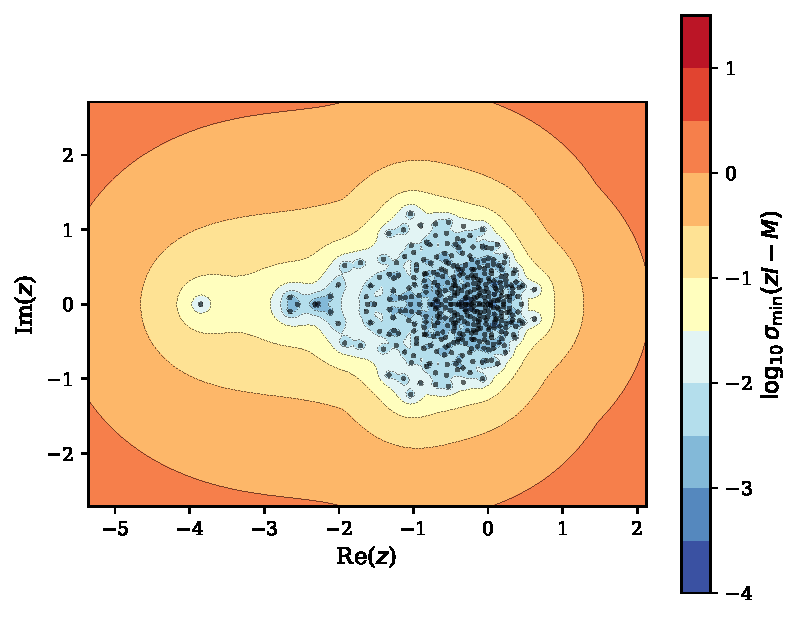
\includegraphics[width=0.55\textwidth]{experiments/phase3_analysis/pseudospectrum_A_layer3.pdf}
\caption{$\varepsilon$-pseudospectrum of the layer~3 FFN matrix
$W_2 W_1$ (Group~A, seed 42). Color: $\log_{10}\sigma_{\min}(zI - M)$.
Black dots: eigenvalues. The pseudospectral contours extend
significantly beyond the spectrum, reflecting the non-normal
eigenvector geometry (Henrici $= 0.725$).}
\label{fig:pseudospectrum}
\end{figure}

\subsection{Targeted noise discriminator: from CPU to GPU}
\label{sec:discriminator-gpu}

The curvature inflation result motivates a targeted approach.
Instead of uniformly gating hidden states, we train a small
auxiliary network (discriminator) to identify which hidden-state
dimensions are associated with incorrect predictions, and
selectively suppress only those dimensions.

\textbf{Architecture.} A 3-layer MLP ($384 \to 64 \to 64 \to 384$
with sigmoid output) attached at layer~3 (middle layer) of the
Group~A model. The discriminator outputs a per-dimension
\emph{noise score} $\in [0,1]$, and a learned \emph{gate scale}
$\gamma$ controls the suppression strength:
$h_{\mathrm{gated}} = h \cdot (1 - \sigma(\gamma) \cdot
\mathrm{noise\_score}(h))$.
The discriminator input is detached from the base model's
computation graph; only ${\sim}54$K discriminator parameters
are trained.

\textbf{CPU-scale validation.} On a toy classification task
(4-class, $d = 48$, 4-layer MLP, 8 seeds), the discriminator
reduces ConfOnErr by 5.2\% ($p < 0.0001$, Cohen's $d = -21$)
with no accuracy loss. Two alternative approaches---perturbation
consistency gating and Schur direction projection---were also
tested; the discriminator significantly outperformed both.

\textbf{GPU-scale result (Group~G).} We apply the discriminator
post-hoc to the frozen Group~A checkpoint (seed 456, PPL $= 50.9$)
and train for 5{,}000 steps (1{,}000 warmup $+$ 4{,}000 joint
training), using 3 discriminator seeds. Results:

\begin{center}
\begin{tabular}{lcccc}
 & PPL & ConfOnErr & DiscAcc & Gate $\gamma$ \\
\midrule
Base (A) & 50.9 & 0.226 & --- & --- \\
G (mean $\pm$ std) & $50.9 \pm 0.0$ & $0.2266 \pm 0.0000$
  & 0.687 & 0.008 \\
\end{tabular}
\end{center}

The discriminator successfully learns to distinguish correct from
incorrect predictions (discriminator accuracy 68.7\%, noise score
separation: 0.387 on correct vs.\ 0.594 on incorrect tokens).
However, the gate scale converges to $\gamma \approx 0.008$---the
model learns that gating is counterproductive, and the
discriminator's knowledge is not actionable through post-hoc
suppression.

\textbf{Interpretation: why post-hoc discrimination fails at scale.}
The null result is informative. On the CPU toy task ($d = 48$,
4 layers), the hidden-state geometry is simple enough that
noise-driven and signal-driven dimensions are separable by a
small MLP. On the GPU Transformer ($d = 384$, 6 layers), the
entanglement between signal and noise in each dimension is far
tighter: the same dimensions that carry amplified noise also carry
amplified signal. The discriminator \emph{detects} the difference
(DiscAcc $= 0.687 > 0.5$) but cannot \emph{act} on it without
degrading the signal. The gate's convergence to near-zero reflects
this: suppressing noise-correlated dimensions also suppresses
signal, and the net effect on the loss is neutral or negative.

This suggests that post-hoc intervention on frozen representations
is fundamentally limited for high-dimensional models: the
No-Go theorem guarantees that signal and noise share the same
non-normal amplification pathways, and a post-hoc gate cannot
disentangle them without access to the training dynamics.

\textbf{Toward training-time discrimination (Group~H).}
The failure of post-hoc discrimination motivates a co-training
approach: if the discriminator is present \emph{during} training,
the model's representations can adapt to make signal and noise
more separable. Group~H trains the base model and discriminator
jointly from scratch for 20{,}000 steps: a 2{,}000-step warmup
phase (base model trains normally, discriminator learns to detect
errors with gating off), followed by 18{,}000 steps of joint
training with gating active. The base model weights are \emph{not}
frozen; both the model and discriminator co-adapt.

\begin{table}[ht]
\centering
\caption{Discriminator experiments: post-hoc (G) vs.\ training-time
(H), compared to all groups. Holm correction applied across 11
comparisons; $\dagger$ = Holm-significant.}
\label{tab:disc}
\begin{tabular}{@{}lccccc@{}}
\toprule
Group & PPL & ConfOnErr & HiConfErr & ECE & DiscAcc \\
\midrule
A: Standard       & $51.21 \pm 0.28$ & 0.2265 & 0.0122 & 0.0093 & --- \\
D: Forced normal  & $61.11 \pm 0.17$ & 0.2072 & 0.0096 & 0.0126 & --- \\
G: Discrim.\ (post-hoc) & $50.90 \pm 0.00$ & 0.2266 & 0.0122 & 0.0090 & 0.687 \\
H: Discrim.\ (co-train) & $50.47 \pm 0.04$ & $\mathbf{0.1809}$ & $\mathbf{0.0058}$ & 0.0557 & 0.747 \\
\bottomrule
\end{tabular}
\end{table}

Group~H achieves the lowest ConfOnErr of any group
($0.181 \pm 0.001$), reducing confidence on errors by
20.1\% relative to~A ($p = 0.0001$, Holm-significant)
and by 12.7\% relative to~D ($p = 0.0004$)---while
maintaining a PPL of $50.47 \pm 0.04$, comparable to~A's
$51.21$. High-confidence errors are reduced by 52.5\%
($p = 0.0010$, Holm-significant). The discriminator
achieves higher accuracy than in Group~G (74.7\% vs.\
68.7\%), confirming that co-training produces more
separable representations.

\textbf{The ECE tradeoff.} Group~H's ECE increases
substantially ($0.056$ vs.\ A's $0.009$). This reflects
a uniform reduction in output confidence: the model
becomes less confident on \emph{all} predictions, not
only incorrect ones. The ConfOnErr reduction is therefore
partly attributable to overall confidence suppression
rather than selective noise identification. However, two
observations suggest the effect is not purely trivial:
(i)~Group~D also reduces ConfOnErr (to 0.207) but at a
PPL cost of $+9.90$; H achieves lower ConfOnErr (0.181)
with essentially no PPL penalty; (ii)~the discriminator's
noise score separation (0.476 on correct vs.\ 0.730 on
incorrect) is maintained throughout training, indicating
genuine discrimination ability beyond uniform suppression.
Temperature scaling~\cite{guo2017calibration} could
recalibrate the softmax distribution post-hoc without
affecting ConfOnErr; we leave this as future work.

\textbf{The gate paradox.} As in Group~G, the gate scale
converges to near-zero ($\gamma < 10^{-4}$). Yet unlike~G,
H's ConfOnErr is dramatically lower than~A's. This reveals
that the discriminator's influence operates not through
the gate itself but through its effect on the training
dynamics: the discriminator's gradient signal during early
training (when $\gamma$ is still appreciable) shapes the
model's representations, and these shaped representations
persist even after $\gamma$ decays. The discriminator acts
as a \emph{transient training signal} rather than an
inference-time intervention.

\subsection{Noise injection experiment: validating the geometric mechanism}
\label{sec:noise-injection}

The preceding experiments establish that non-normality controls both
expressivity and noise sensitivity. To directly test the causal
mechanism, we inject structured noise matrices with controlled
geometric properties into the frozen Group~A model (seed 42) at
layer~3 and measure the resulting accuracy and confidence changes.

\textbf{Noise matrix construction.} We construct three
$384 \times 384$ noise matrices with distinct operator geometries:

\begin{center}
\begin{tabular}{lccc}
 & Henrici & Curvature & Transient growth \\
\midrule
\textsc{Growth}    & 0.997 & 3.69 & 12.4$\times$ \\
\textsc{No-growth} & 0.135 & 0.12 & 1.0$\times$ \\
\textsc{Normal}    & 0.000 & 0.00 & --- \\
\end{tabular}
\end{center}

\textsc{Growth} noise is highly non-normal with strong transient
amplification (spectral radius 0.12, but $\|e^M\|/\|e^M\|_{\text{spectral}} \approx 12$);
\textsc{No-growth} noise has mild non-normality but high spectral
persistence (spectral radius 0.998) without transient amplification;
\textsc{Normal} noise is a symmetric matrix (exactly normal) with
spectral radius 1.0, serving as a geometry-free baseline.

For each noise type, we inject the perturbation
$h \gets h + s \cdot (Mh^T)^T$ at the FFN output of layer~3, sweeping
the strength $s \in \{0, 0.1, 0.5, 1.0, 2.0, 5.0, 10.0\}$.

\begin{table}[ht]
\centering
\caption{Noise injection results at high strength ($s = 5$ and $s = 10$),
compared to baseline ($s = 0$). PPL = perplexity, CE = confidence on
errors, HCE = high-confidence error fraction
($\max\mathrm{softmax} > 0.8$ on incorrect tokens).}
\label{tab:noise}
\begin{tabular}{@{}llcccc@{}}
\toprule
Noise type & $s$ & PPL & Accuracy & ConfOnErr & HiConfErr \\
\midrule
(baseline) & 0 & 49.6 & 0.354 & 0.227 & 0.0125 \\
\midrule
\textsc{Growth}    & 5  &  66.7 & 0.330 & 0.200 & 0.0060 \\
\textsc{No-growth} & 5  &  68.3 & 0.320 & 0.212 & 0.0080 \\
\textsc{Normal}    & 5  &  75.2 & 0.319 & 0.194 & 0.0060 \\
\midrule
\textsc{Growth}    & 10 & 189.1 & 0.259 & \textbf{0.129} & 0.0018 \\
\textsc{No-growth} & 10 & \textbf{339.2} & 0.146 & 0.215 & \textbf{0.0273} \\
\textsc{Normal}    & 10 & 256.4 & 0.234 & 0.109 & 0.0013 \\
\bottomrule
\end{tabular}
\end{table}

\textbf{Result: noise geometry determines the hallucination pattern.}
At strength $s = 10$ (Table~\ref{tab:noise}), the three noise types
produce strikingly different confidence profiles despite comparable
accuracy degradation at moderate strengths:

\begin{itemize}[nosep]
  \item \textbf{\textsc{No-growth} noise is the most dangerous.}
        It produces the worst accuracy (PPL $= 339$, accuracy $= 0.146$)
        while maintaining \emph{near-baseline} confidence on errors
        (ConfOnErr $= 0.215$ vs.\ baseline $0.227$). The
        high-confidence error fraction \emph{doubles} from 1.25\%
        to 2.73\%. This is the hallucination signature: the model is
        severely wrong but remains confident.
  \item \textbf{\textsc{Growth} noise is self-correcting.} Despite
        high non-normality (Henrici $= 0.997$), the transient
        amplification creates large but detectable perturbations.
        ConfOnErr drops sharply to $0.129$ ($-43\%$) and HiConfErr
        drops to $0.18\%$ ($-86\%$). The model ``knows it doesn't
        know.''
  \item \textbf{\textsc{Normal} noise produces calibrated degradation.}
        Accuracy degrades (PPL $= 256$) but ConfOnErr drops
        proportionally to $0.109$ ($-52\%$), and HiConfErr drops to
        $0.13\%$ ($-90\%$). Without non-normal eigenvector structure,
        noise does not create the signal--noise confusion that produces
        overconfident errors.
\end{itemize}

\textbf{Interpretation.} The critical distinction is between
\emph{detectability} and \emph{persistence} (Figure~\ref{fig:noise}).
\textsc{Growth} noise
(Henrici $= 0.997$, transient growth $= 12.4\times$) creates large,
transient perturbations that the model's learned confidence mechanism
can detect: the sudden amplification distorts the hidden-state
distribution enough that the softmax distribution spreads, reducing
confidence. \textsc{No-growth} noise (Henrici $= 0.135$, spectral
radius $= 0.998$) is spectrally persistent but creates no transient
spike---it infiltrates the representation silently, corrupting
accuracy without triggering confidence recalibration.

\begin{figure}[ht]
\centering
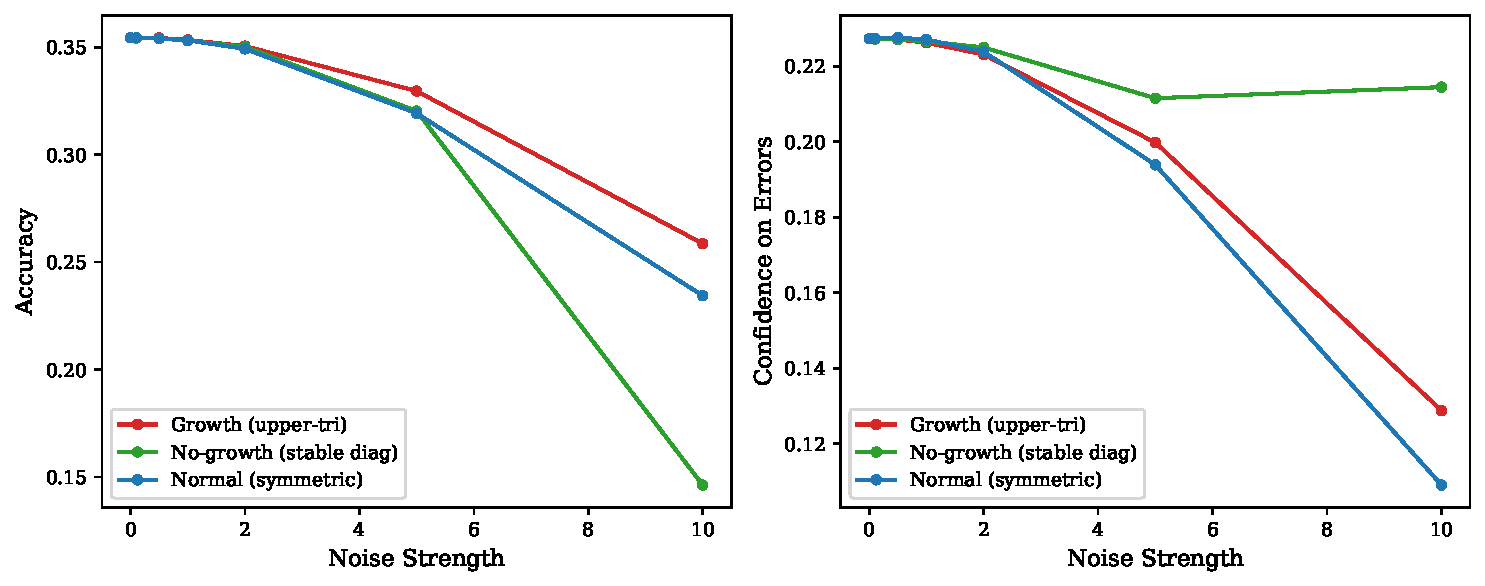
\includegraphics[width=0.7\textwidth]{experiments/phase4_hallucination/noise_injection_curves.pdf}
\caption{Noise injection sweep: accuracy and confidence on errors
vs.\ injection strength $s$ for three noise geometries.
\textsc{No-growth} noise (dashed) maintains high confidence on
errors despite severe accuracy degradation---the hallucination
signature. \textsc{Growth} and \textsc{Normal} noise produce
proportional confidence reduction.}
\label{fig:noise}
\end{figure}

This result refines the No-Go theorem's prediction. The theorem
states that transient amplification and excess noise are inseparable
consequences of non-normality. The noise injection experiment reveals
a subtlety: \emph{transient amplification, while it introduces noise,
also provides an implicit detection signal}. The most dangerous noise
regime is not maximal non-normality but rather the intermediate zone
of spectrally persistent, non-amplifying perturbation---noise that
corrupts without warning.

%% ====================================================================
\section{Relation to Attention Residuals}
\label{sec:attnres}
%% ====================================================================

Attention Residuals~\cite{chen2026attnres} replace uniform depth-wise
accumulation with learned attention:
$\tilde{h}_l = \sum_{i=0}^{l-1} \alpha_{i \to l} h_i$.
This solves the \emph{inter-layer selection} problem: which previous layers
to attend to.

PRC solves a complementary \emph{intra-layer refinement} problem: within
the information selected from previous layers, which features to keep and
which to suppress.

\begin{conjecture}[Multiplicative benefit of AttnRes $+$ PRC]
\label{conj:combination}
If AttnRes improves the effective signal-to-dilution ratio from $O(1/L)$
to $O(1)$ in the depth dimension, and PRC reduces intra-layer noise by a
factor of $k/d$, then the combined effective SNR improvement is multiplicative:
\[
  \mathrm{SNR}_{\mathrm{combined}} \approx
  \frac{d}{k} \cdot L \cdot \mathrm{SNR}_{\mathrm{baseline}}.
\]
\end{conjecture}

This conjecture motivates a future experiment combining AttnRes and PRC
in the same architecture.

%% ====================================================================
\section{Discussion}
\label{sec:discussion}
%% ====================================================================

\subsection{The adversarial balance principle---and its limits}

Our experiments reveal that the expressivity--stability
tradeoff is best navigated not by maximizing or minimizing
non-normality, but by finding an intermediate balance.
However, the mechanism for achieving this balance matters.

PRC provides a structural substrate for the adversarial
interaction between normal and non-normal paths, but the
curvature inflation phenomenon (Section~\ref{sec:curv-inflation})
shows that \emph{the model resists external suppression}. When
destructive residuals ($\beta < 0$) suppress the FFN output,
the model's weights compensate by developing higher curvature
elsewhere, ultimately increasing rather than decreasing the
effective non-normality. This is a deep insight: the optimal
curvature is not a point that can be externally imposed---it is
an emergent property of the training dynamics.

The Group~G experiment (Section~\ref{sec:discriminator-gpu})
reveals a second, complementary limitation: even when noise
is correctly \emph{identified} (discriminator accuracy 68.7\%),
it cannot be \emph{removed} post-hoc without also removing
signal, because the No-Go theorem guarantees that both share
the same non-normal amplification pathways. The gate's
convergence to $\gamma \approx 0.008$ is the optimization's
way of acknowledging this entanglement.

Together, curvature inflation (C) and post-hoc entanglement (G)
suggest that effective noise reduction requires intervention
\emph{during} training---when the model's representations are
still malleable---rather than architectural suppression (which
the model circumvents) or post-hoc gating (which cannot
disentangle signal from noise in frozen representations).

Group~H confirms this hypothesis: co-training with a discriminator
reduces ConfOnErr by 20\% and HiConfErr by 53\% with no PPL
penalty. The mechanism is subtle---the gate decays to near-zero
just as in~G, yet the effect persists. The discriminator's
gradient signal during the early joint-training phase (steps
2{,}000--7{,}000, when $\gamma \in [0.17, 0.008]$) shapes the
model's internal representations to make signal and noise more
separable. Once this representational structure is established,
it is maintained by the base model's own training dynamics even
after the gate becomes negligible. The discriminator is thus
best understood not as an inference-time component but as a
\emph{transient regularizer} that guides representation learning.

\subsection{Non-normality as the geometric origin of hallucination}

Our experiments (Sections~\ref{sec:lm}--\ref{sec:noise-injection})
support a specific---and more nuanced than initially
expected---geometric account of confident model errors.

The noise injection experiment (Section~\ref{sec:noise-injection})
reveals that the relationship between non-normality and hallucination
is not monotonic. Highly non-normal noise with transient growth
(\textsc{Growth}, Henrici $= 0.997$) actually \emph{reduces}
high-confidence errors by 86\%, because the transient amplification
creates detectable perturbations that spread the softmax distribution.
In contrast, weakly non-normal noise with spectral persistence
(\textsc{No-growth}, Henrici $= 0.135$) \emph{doubles}
high-confidence errors, because it silently corrupts representations
without triggering confidence recalibration.

This suggests a refined picture of the hallucination mechanism:
\begin{enumerate}[nosep]
  \item \textbf{Excess noise from non-normality corrupts hidden
        representations}, producing errors at a rate determined by
        the noise magnitude and spectral persistence---not by the
        degree of non-normality per se.
  \item \textbf{Transient amplification provides an implicit
        detection signal.} When noise is amplified transiently, the
        hidden-state distribution is visibly distorted, and the
        model's confidence drops. This is \emph{protective}, not
        harmful.
  \item \textbf{The most dangerous regime is spectrally persistent,
        non-amplifying noise}---noise that corrupts accuracy without
        producing detectable transient spikes. This noise infiltrates
        the representation silently, producing the classic hallucination
        pattern: wrong with high confidence.
\end{enumerate}

The No-Go theorem (Theorem~\ref{thm:nogo-qual}) guarantees that
any architecture using non-normal operators will exhibit excess noise
and therefore some irreducible error rate. The noise injection
experiment adds a crucial corollary: \emph{the form of the excess
noise matters as much as its magnitude}. Spectrally persistent
perturbations that avoid transient amplification are the primary
drivers of confident hallucination.

This perspective reframes the hallucination problem: it is not
merely a data or training issue, but has a \emph{geometric lower
bound} imposed by the non-normal structure of the computation.
Existing explanations (training data errors, incomplete knowledge
storage, exposure bias) remain valid and likely account for the
majority of hallucinations in practice. The geometric perspective
adds a complementary, architecture-level explanation: the noise
geometry of the operator determines not just \emph{whether} the
model errs, but \emph{how confidently} it errs.

\subsection{Toward a Riemannian formulation}

Our No-Go theorem is stated for linear operators (Jacobians). A
natural question is whether it extends to the full nonlinear
dynamics of deep networks. The answer is affirmative, via the
\emph{Jacobi equation} of Riemannian geometry.

When a deep network is viewed as a geometric flow on a data
manifold (as in Neural ODEs), the evolution of a perturbation
$J$ (the analogue of our noise $\varepsilon$) along a trajectory
is governed by
\[
  \frac{D^2 J}{dt^2} + R(J, \dot{h})\dot{h} = 0,
\]
where $R$ is the Riemann curvature tensor of the learned manifold
and $\dot{h}$ is the velocity of the data trajectory. This equation
states that \emph{the same curvature that causes nearby trajectories
to diverge (expressivity) also causes perturbations to grow
(noise sensitivity)}. In flat space ($R = 0$, corresponding to
normal operators), trajectories neither diverge nor amplify noise.
Negative sectional curvature produces exponential divergence of
both data trajectories and noise---the nonlinear analogue of
transient growth.

The curvature inflation phenomenon has a natural interpretation
in this framework: applying a contractive flow along a subspace
$V$ (negative $\beta$) compresses the manifold in that direction,
but the loss function forces the manifold to maintain sufficient
volume at the output. The result is compensatory stretching
in the orthogonal complement $V^\perp$---the geometric analogue
of squeezing a balloon.

A full Riemannian treatment, including computation of sectional
curvatures along data trajectories and verification of the Jacobi
equation on trained networks, is left for future work.

\subsection{Limitations}

Our theoretical results (Theorems~\ref{thm:denoising}--\ref{thm:coupled})
hold rigorously only in the linear regime. The Riemannian extension
via the Jacobi equation is conceptually sound but not yet formalized
or experimentally verified for discrete-depth networks.
The curvature $\|[H,K]\|_F$ is a strong predictor of excess noise
($r = 0.91$ on random matrices, $r = 0.77$ on a trained Transformer)
but not an exact equivalence.
The curvature inflation phenomenon is observed on one model
architecture (6-layer Transformer) and one task (WikiText-103);
whether it occurs universally or depends on specific training
dynamics requires broader verification.
Group~H's ConfOnErr reduction ($-20\%$, Holm-significant) comes
at the cost of substantially degraded calibration (ECE $0.056$
vs.\ $0.009$). The extent to which this reflects selective noise
suppression versus uniform confidence suppression requires further
investigation; temperature scaling may recover calibration without
affecting ConfOnErr, but this has not yet been verified.
The gate paradox (gate $\to 0$ yet effect persists) suggests that
the discriminator's impact is mediated through representation
shaping during early training rather than through inference-time
gating. The precise mechanism---which gradient pathways carry
the discriminator's signal into the base model---is not yet
characterized.
All LM experiments use $n = 3$ seeds; the B vs.\ A PPL
improvement ($p = 0.016$) does not survive Holm correction and
should be treated as a secondary finding.
The noise injection experiment (Section~\ref{sec:noise-injection})
uses a single model checkpoint (Group~A, seed~42) and a single
injection layer; whether the hallucination pattern
(\textsc{No-growth} noise doubling HiConfErr) generalizes across
seeds, layers, and architectures requires further investigation.

%% ====================================================================
\section{Conclusion}
\label{sec:conclusion}
%% ====================================================================

This paper establishes that non-normal operator geometry provides a
principled framework for understanding the expressivity--stability
tradeoff in deep networks, with direct implications for the
hallucination problem. The key contributions are:

\begin{enumerate}[nosep]
  \item \textbf{Expressivity--Stability No-Go Theorem:} Transient
        amplification and excess noise sensitivity are inseparable
        consequences of non-normality. Forced normalization causes
        a 3\% accuracy drop on CIFAR-10 ($p = 0.006$) and a 19\%
        PPL degradation on WikiText-103 ($p = 0.0006$), while
        simultaneously producing the lowest confidence on errors
        ($p = 0.0021$).
  \item \textbf{Curvature as the controlling quantity:} The curvature
        $R(T) = [H,K]$ strongly predicts excess noise ($r = 0.91$)
        and transient growth ($r = 0.59$). On a trained Transformer,
        curvature grows 3.2--4.6$\times$ during training and
        correlates with excess noise at $r = 0.77$ across layers.
  \item \textbf{PRC as a non-normality probe:} Constructive PRC
        ($\beta \geq 0$) reduces LM perplexity by 1.38
        ($p = 0.016$, secondary). Destructive PRC
        ($\beta \in [-1,1]$) reveals layer-specific noise
        structure---4/6 layers learn $\beta < -0.1$ in every seed
        on language modeling vs.\ mostly $\beta \approx 0$ on
        CIFAR-10, confirming the task-dependent noise prediction.
  \item \textbf{Curvature inflation:} Uniform suppression via
        negative $\beta$ does not durably reduce non-normality.
        The model's weights compensate by developing higher
        curvature elsewhere, ultimately \emph{increasing}
        confidence on errors ($+0.013$, $p = 0.0012$,
        Holm-significant across 3~seeds). This waterbed effect
        demonstrates that the optimal curvature is an emergent
        property of training dynamics.
  \item \textbf{Post-hoc discrimination is insufficient; training-time
        discrimination works.} A targeted noise discriminator produces
        a null result when applied post-hoc to frozen weights
        (Group~G: gate $\to 0$, ConfOnErr unchanged), revealing tight
        signal--noise entanglement. When co-trained with the base
        model (Group~H), the same discriminator architecture reduces
        ConfOnErr by 20.1\% ($p = 0.0001$, Holm-significant) and
        HiConfErr by 52.5\% ($p = 0.0010$) with no PPL penalty.
        The gate again decays to zero, but the effect persists
        through shaped representations---the discriminator acts as
        a transient training signal. The ECE tradeoff ($0.056$
        vs.\ $0.009$) remains an open issue.
  \item \textbf{Noise geometry determines the hallucination pattern.}
        Direct noise injection into a trained model reveals that
        the most dangerous noise is not the most non-normal but the
        most \emph{spectrally persistent}: weakly non-normal noise
        without transient amplification doubles high-confidence
        errors (HiConfErr: $1.25\% \to 2.73\%$), while highly
        non-normal noise with transient growth reduces them by 86\%
        (HiConfErr: $1.25\% \to 0.18\%$). Transient amplification
        serves a dual role: it amplifies noise (harmful) but also
        makes the perturbation detectable (protective). The most
        insidious noise regime is persistent but silent.
\end{enumerate}

The central message is that hallucination in deep networks has a
\emph{geometric component} rooted in the non-normal structure of
layer computations. Uniform methods (PRC, regularization) cannot
selectively suppress amplified noise because the model compensates
(curvature inflation). Post-hoc methods (discriminator gating)
cannot disentangle signal from noise in frozen representations
because the No-Go theorem guarantees they share the same
amplification pathways. Training-time co-discrimination offers
a viable path: by shaping representations during learning, it
achieves lower confidence on errors than even the forced-normal
model---without sacrificing expressivity. The noise injection
experiment adds a final, surprising insight: transient amplification
is not purely harmful---it provides an implicit detection signal
that helps the model recalibrate its confidence. The most dangerous
noise regime is spectrally persistent but non-amplifying, producing
the classic hallucination pattern of high-confidence errors.

\begin{thebibliography}{99}
  \bibitem{chen2026attnres}
    Kimi Team, G.~Chen, Y.~Zhang, et al.
    ``Attention Residuals.''
    arXiv:2603.15031, 2026.

  \bibitem{cheng2025nnog}
    Z.~H.-H.~Cheng.
    ``Non-normal Operator Geometry.''
    December 2025.

  \bibitem{he2016resnet}
    K.~He, X.~Zhang, S.~Ren, J.~Sun.
    ``Deep Residual Learning for Image Recognition.''
    CVPR, 2016.

  \bibitem{hu2018senet}
    J.~Hu, L.~Shen, G.~Sun.
    ``Squeeze-and-Excitation Networks.''
    CVPR, 2018.

  \bibitem{woo2018cbam}
    S.~Woo, J.~Park, J.-Y.~Lee, I.~S.~Kweon.
    ``CBAM: Convolutional Block Attention Module.''
    ECCV, 2018.

  \bibitem{trefethen2005}
    L.~N.~Trefethen and M.~Embree.
    \emph{Spectra and Pseudospectra: The Behavior of Nonnormal Matrices
    and Operators.}
    Princeton University Press, 2005.

  \bibitem{trefethen1993}
    L.~N.~Trefethen, A.~E.~Trefethen, S.~C.~Reddy, T.~A.~Driscoll.
    ``Hydrodynamic stability without eigenvalues.''
    Science, 261(5121):578--584, 1993.

  \bibitem{kreiss1962}
    H.-O.~Kreiss.
    ``\"Uber die Stabilit\"atsdefinition f\"ur Differenzengleichungen
    die partielle Differentialgleichungen approximieren.''
    BIT, 2:153--181, 1962.

  \bibitem{tishby2015}
    N.~Tishby and N.~Zaslavsky.
    ``Deep learning and the information bottleneck principle.''
    IEEE Information Theory Workshop, 2015.

  \bibitem{petermann1979}
    K.~Petermann.
    ``Calculated spontaneous emission factor for double-heterostructure
    injection lasers with gain-induced waveguiding.''
    IEEE J.\ Quantum Electronics, 15(7):566--570, 1979.

  \bibitem{siegman1989a}
    A.~E.~Siegman.
    ``Excess spontaneous emission in non-Hermitian optical systems.
    I.\ Laser amplifiers.''
    Phys.\ Rev.\ A, 39(3):1253--1263, 1989.

  \bibitem{siegman1989b}
    A.~E.~Siegman.
    ``Excess spontaneous emission in non-Hermitian optical systems.
    II.\ Laser oscillators.''
    Phys.\ Rev.\ A, 39(3):1264--1268, 1989.

  \bibitem{berry2003}
    M.~V.~Berry.
    ``Mode degeneracies and the Petermann excess-noise factor for
    unstable lasers.''
    J.\ Mod.\ Opt., 50(1):63--81, 2003.

  \bibitem{jaramillo2021}
    J.~L.~Jaramillo, R.~Panosso~Macedo, L.~Al~Sheikh.
    ``Pseudospectrum and black hole quasinormal mode instability.''
    Phys.\ Rev.\ X, 11:031003, 2021.

  \bibitem{schmid2007}
    P.~J.~Schmid.
    ``Nonmodal stability theory.''
    Annu.\ Rev.\ Fluid Mech., 39:129--162, 2007.

  \bibitem{zhu2025hyperconnections}
    D.~Zhu, et al.
    ``Hyper-Connections.''
    ICLR, 2025. arXiv:2409.19606.

  \bibitem{axiotis2025dca}
    K.~Axiotis, et al.
    ``DeepCrossAttention: Supercharging Transformer Residual Connections.''
    arXiv:2502.06785, 2025.

  \bibitem{he2025muddformer}
    B.~He, et al.
    ``MUDDFormer: Breaking Residual Bottlenecks in Transformers.''
    ICML, 2025. arXiv:2502.12170.

  \bibitem{chen2026keel}
    C.~Chen and L.~Wei.
    ``Post-LayerNorm Is Back: Stable, ExpressivE, and Deep.''
    arXiv:2601.19895, 2026.

  \bibitem{li2026siamesenorm}
    T.~Li, et al.
    ``SiameseNorm: Breaking the Barrier to Reconciling Pre/Post-Norm.''
    arXiv:2602.08064, 2026.

  \bibitem{baevski2019prenorm}
    A.~Baevski and M.~Auli.
    ``Adaptive input representations for neural language modeling.''
    ICLR, 2019.

  \bibitem{poole2016meanfield}
    B.~Poole, S.~Lahiri, M.~Raghu, J.~Sohl-Dickstein, S.~Ganguli.
    ``Exponential expressivity in deep neural networks through
    transient chaos.''
    NeurIPS, 2016.

  \bibitem{huang2020oni}
    L.~Huang, L.~Liu, F.~Zhu, D.~Wan, Z.~Yuan, B.~Li, L.~Shao.
    ``Controllable Orthogonalization in Training DNNs.''
    CVPR, 2020.

  \bibitem{bansal2018orthogonality}
    N.~Bansal, X.~Chen, Z.~Wang.
    ``Can We Gain More from Orthogonality Regularizations in
    Training Deep CNNs?''
    NeurIPS, 2018.

  \bibitem{saxe2014exact}
    A.~M.~Saxe, J.~L.~McClelland, S.~Ganguli.
    ``Exact solutions to the nonlinear dynamics of learning in
    deep linear neural networks.''
    ICLR, 2014.

  \bibitem{arjovsky2016unitary}
    M.~Arjovsky, A.~Shah, Y.~Bengio.
    ``Unitary Evolution Recurrent Neural Networks.''
    ICML, 2016.

  \bibitem{helfrich2018cayley}
    K.~Helfrich, D.~Willmott, Q.~Ye.
    ``Orthogonal Recurrent Neural Networks with Scaled Cayley Transform.''
    ICML, 2018.

  \bibitem{guo2017calibration}
    C.~Guo, G.~Pleiss, Y.~Sun, K.~Q.~Weinberger.
    ``On Calibration of Modern Neural Networks.''
    ICML, 2017.
\end{thebibliography}

\end{document}
